%!TEX root = ../thesis.tex

\chapter{TRANSITIVITY choices in the Forum} \label{chap:experiential}

In Chapter \ref{chap:interpersonal}, I analysed \sctext{Mood} and \sctext{Modality} features of the \gls{corpus}, discussing findings with respect to interpersonal meaning\hyp{}making in the \glslink{Forum}{community}. This chapter uses similar methods to focus on experiential meanings, and their realisation within \sctext{Transitivity} choices. This allows observation of how inner (mental) and outer (physical) states are represented by \gls{Forum} \glspl{member}. \sctext{Transitivity} analysis of a clause involves distinguishing between Process Types or ergativity (represented in the main verbal group), as well as participants (the arguments of the verbal group) and circumstances (which modify the meaning made by the process). In this chapter, the analysis of participants is performed first, and processes second. That said, more delicate queries often involve consideration of both, as well as their attendant modifiers and circumstances. Rather than using constituency grammar, this part of the investigation relies on dependency annotations, which more closely model the \sctext{Transitivity} system \cite{costetchi_method_2013}. Collapsed, conjunction\hyp{}processed dependencies are used in almost almost all cases \cite[see][]{manning_stanford_2014}.

For both participants and processes, the workflow is similar. Heads of groups are extracted from the \gls{corpus} and transformed into relative frequencies and keyword tables. Linear\hyp{}regression based sorting is used to determine which results are on increasing, decreasing, static and turbulent trajectories, in terms of both relative frequency and keyness. A subset of results undergoing obvious trajectory shifts are then analysed in greater detail, by probing their lexicogrammatical behaviour, and by concordancing. Profiles for these results, and for concepts indexed by sets of related lexis, are constructed in order to highlight differences in the way they are deployed in the subcorpora of each \gls{corpus} under investigation.

Because of the strong methodological focus of the thesis, results are typically presented without manual removal of parsing errors, or of phenomena that are vague or difficult to interpret. Where necessary, the cause of errors is discussed before moving forward to analysis of the generated result. The argument being advanced, both here and in later chapters, is that doing discourse analysis or \gls{CL}\slash \gls{CADS} can be automated to a greater extent than it thus far has been: targeted searches of the \gls{lexicogrammar}, exclusion of instances based on non\hyp{}arbitrary information, and trajectory\hyp{}based sorting can leave the analyst with summarised lexicogrammatical information with relatively obvious links to \glspl{discourse-semantic}. Unedited result lists are therefore presented in order to demonstrate both the promise of partially automated \gls{CL} methods and the seriousness of limitations in the method that are discussed in Chapters \ref{chap:discuss-bp} and \ref{chap:implications}.

\section{Participants}

To locate participants, a \gls{corpus} can be searched for the lemma forms of dependency nodes of particular types, roughly corresponding to distinctions made within the \gls{SFG}. For participant, the corresponding labels are \emph{acomp}, \emph{agent}, \emph{appos}, \emph{csubj}, \emph{csubjpass}, \emph{dobj}, \emph{iobj}, \emph{nsubj}, \emph{nsubjpass} and \emph{xsubj}. There are some inconsistencies between the grammars that are difficult to resolve, however: as one example, the Universal Dependency grammar used by \texttt{Stanford CoreNLP} annotates the Range in a process\hyp{}range configuration (\emph{I took a shower}) with the same label as it does a Goal (\emph{I built a shower}). Even so, there is a great deal of overlap between the grammars, especially in the case of the general distinction between process and participant.

% Relative frequencies of common participant heads in each P subcorpus
    \begin{table}[htb]
    \centering
    \small
    \begin{tabular}{lrrrrrrrrrr}
    
    \toprule
    Subcorpus &     i &   it &   you &   he &  she &  that &  they &   we &  what &  this \\
    \midrule
    $01$ & $32.22$ & $6.31$ & $ 3.48$ & $4.44$ & $2.87$ &  $1.88$ &  $1.84$ & $1.29$ &  $1.61$ &  $1.32$ \\
    $02$ & $30.13$ & $7.10$ & $ 5.09$ & $4.12$ & $2.87$ &  $2.17$ &  $2.16$ & $1.39$ &  $1.63$ &  $1.14$ \\
    $03$ & $29.49$ & $7.40$ & $ 5.46$ & $4.36$ & $2.47$ &  $2.25$ &  $2.18$ & $1.47$ &  $1.73$ &  $1.12$ \\
    $04$ & $28.08$ & $7.49$ & $ 6.44$ & $4.11$ & $2.22$ &  $2.29$ &  $2.25$ & $1.59$ &  $1.68$ &  $1.12$ \\
    $05$ & $27.67$ & $7.62$ & $ 6.91$ & $3.80$ & $2.18$ &  $2.33$ &  $2.35$ & $1.77$ &  $1.77$ &  $1.15$ \\
    $06$ & $26.51$ & $7.54$ & $ 7.52$ & $3.41$ & $2.36$ &  $2.47$ &  $2.29$ & $1.92$ &  $1.71$ &  $1.10$ \\
    $07$ & $26.02$ & $7.69$ & $ 7.82$ & $3.59$ & $2.07$ &  $2.44$ &  $2.38$ & $1.96$ &  $1.66$ &  $1.08$ \\
    $08$ & $25.18$ & $7.76$ & $ 8.05$ & $3.34$ & $2.06$ &  $2.54$ &  $2.32$ & $2.11$ &  $1.70$ &  $1.05$ \\
    $09$ & $21.91$ & $7.79$ & $10.06$ & $3.26$ & $2.39$ &  $2.78$ &  $2.24$ & $2.37$ &  $1.73$ &  $1.05$ \\
    $10$ & $18.65$ & $7.50$ & $11.14$ & $2.96$ & $3.32$ &  $2.88$ &  $2.44$ & $2.30$ &  $1.66$ &  $1.19$ \\
    \bottomrule
    \end{tabular}
    \caption[Relative frequencies of common participant heads]{Relative frequencies of common participant heads at each stage of membership}
    \label{tab:rel_freq_part_stop}
    \end{table}
%
%todo: long sentence :)
Because closed\hyp{}class words have not at this point been excluded, the most common participant heads are generally pronominal (Table \ref{tab:rel_freq_part_stop}). Even so, the shift from first toward second person participants, and the relative stability in third person pronoun usage, are both observable, echoing findings from the investigation of \sctext{Mood} choices, where first and second person pronouns feature prominently as Subjects, and where the latter come to displace the former in veteran talk. Within the domain of interpersonal meaning, the increasing second person as Subject indicated a shift in which interactant is charged with interactive demands. Within the system of \sctext{Transitivity}, however, the shift in meaning is an experiential one: \emph{who is being spoken about} changes over the course of membership, from the self toward the addressee (Table \ref{tab:rel_freq_part_stop}). 

% Keyness of common participant heads in three stages of membership
    \begin{figure}[htb]
    \centering
    \small
    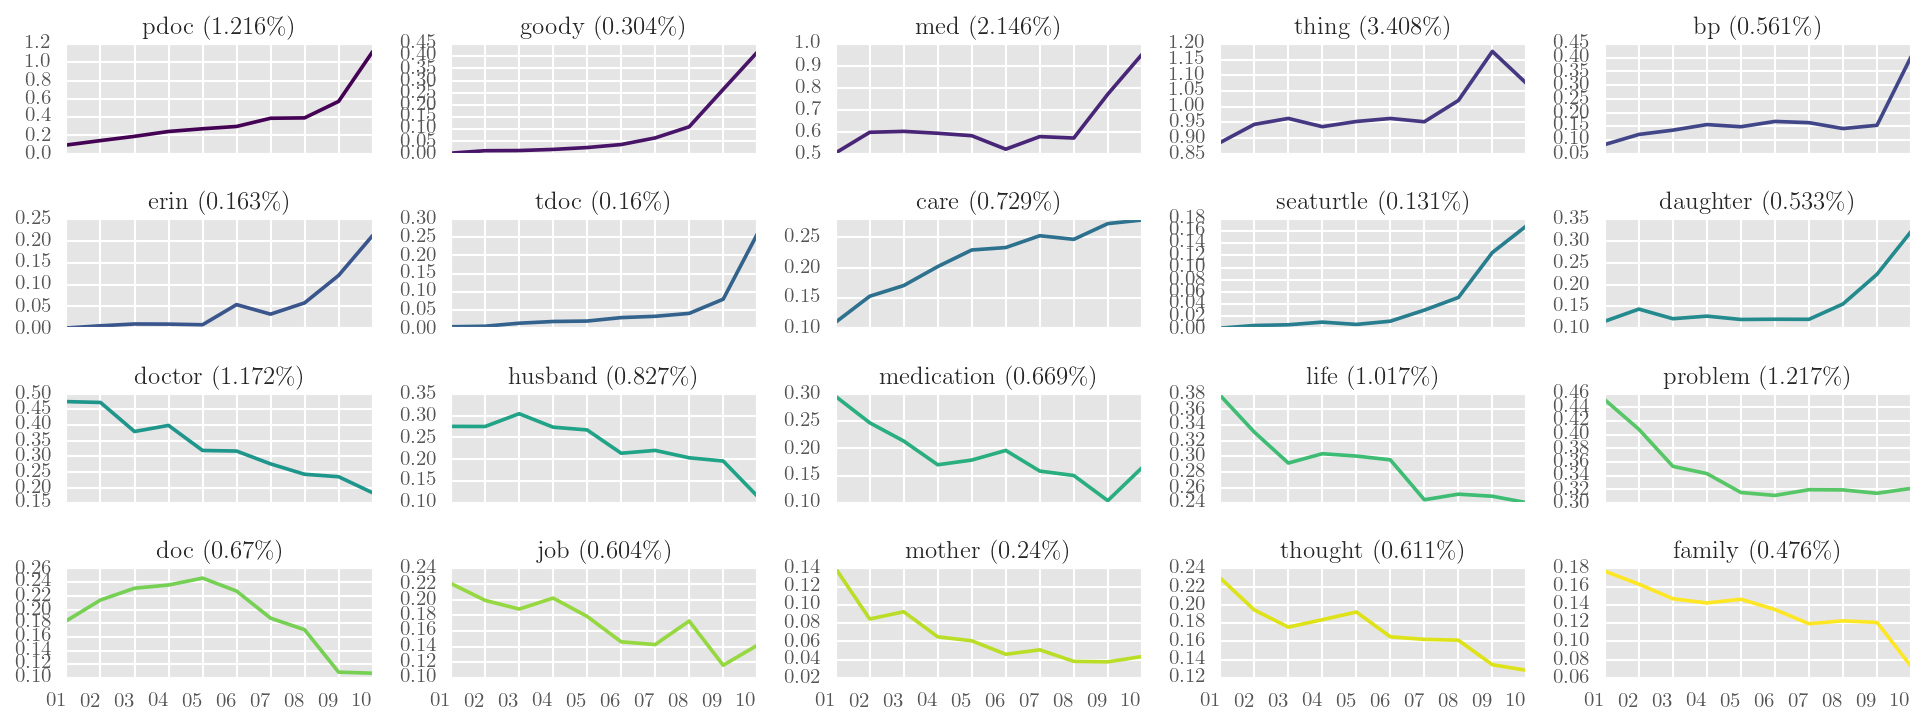
\includegraphics[width=1\textwidth]{../images/part-traj2.png}
    \caption{Trajectory of common participants undergoing change}
    \label{tab:key_part_w_prop}
    \end{figure}
%
Figure \ref{tab:key_part_w_prop} shows the longitudinal trajectories of common open\hyp{}class participant heads, as a percentage of all participants. From the 1000 most common heads, the ten on the most sharply increasing trajectory (top half), and the ten on the most decreasing (bottom half) are shown. Proper nouns denoting veteran \glspl{member} and their family\slash friends (\emph{seaturtle}, \emph{goody}, \emph{erin}, \emph{daughter}) dominate the `increasing' results because veteran \glspl{member} refer to one another and commonly discuss those close to them by name. Similarly, the declining frequency of \emph{husband} and \emph{mother} may have more to do with the particular circumstances of the small group of veteran members than it does to do with a normative value governing the ways in which the world ought to be construed by veteran members of the group. It is important to keep in mind, therefore, that the small sample of veteran \glslink{member}{users} can cause an over\slash under\hyp{}representation of particular participants. Fortunately, removing proper nouns is a trivial task, as they are annotated by \texttt{Stanford CoreNLP} with distinct \gls{POS} tags (\texttt{NNP}\slash \texttt{NNPS}). 

Table \ref{tab:keyunkey-threestage} shows the top participants, excluding pronominal and proper\hyp{}nominal words. It uses log\hyp{}likelihood keyness, rather than simple relative frequency, and collapses the ten subcorpora into three (\emph{Early stages}, \emph{Mid stages} and \emph{Late stages}). Discursive insights become clearer here---negative emotional lexis appears as key in early contributions, while more positive terms and jargon appear as key in later \glspl{post}. Before interpreting these, however, it is important to make note of the issue of parser accuracy, which has an impact on what is classified as a participant. \emph{Welcome} and \emph{thanks}, for example, are in some cases misannotated as participants. This is caused by short, minor clause sentences or sentence fragments, with which the parser model used is unfamiliar. Another problem is that some proper nouns have not been correctly removed: \emph{whiskey} and \emph{kait} are shorthand forms of two veterans' usernames, often misannotated as common nouns or adjectives. The misannotation is caused by the fact that the names may be written without capitalisation in the Forum---uncapitalised proper nouns, like minor clause sentences, are essentially absent in the parser training data.

%\begin{minted}[linenos,breaklines,frame=single,xleftmargin=1cm,breakindent=0em,breaksymbolindentleft=0em]{python}
%parts = corpus.interrogate(search={GF: roles.process,
%                                    F: roles.participant},
%                           exclude={W: wordlists.closedclass,
%                                    P: '^PRP'},
%                           show=[L])
%parts = parts.edit('k', SELF)
%\end{minted}
%

% key and unkey participants in collapsed stages of membership
\begin{table}[p]
    \centering
    \small
    \begin{tabular}{lrlrlr}
     \toprule
    Early stages &        & Mid stages &        & Late stages &         \\
    \midrule
          bipolar & $709.26$ &     person & $114.96$ &        pdoc & $2002.63$ \\
              new & $692.95$ &        doc & $ 97.41$ &        tdoc & $ 735.35$ \\
           doctor & $396.43$ &       hard & $ 87.91$ &         med & $ 339.99$ \\
       medication & $254.38$ &       luck & $ 73.50$ &        glad & $ 316.05$ \\
           mother & $229.52$ &         be & $ 66.70$ &         hug & $ 315.12$ \\
     psychiatrist & $178.40$ &       good & $ 61.09$ &   stability & $ 287.02$ \\
               dr & $161.91$ &        lol & $ 60.07$ &    daughter & $ 278.64$ \\
            swing & $159.18$ &    illness & $ 59.41$ &        able & $ 229.33$ \\
         medicine & $139.93$ &    whiskey & $ 55.67$ &         son & $ 208.47$ \\
          problem & $136.31$ &   kindness & $ 54.89$ &       thing & $ 193.58$ \\
            angry & $135.12$ &  happiness & $ 47.38$ &   important & $ 188.02$ \\
               mg & $125.84$ &         bp & $ 45.07$ &        okay & $ 176.41$ \\
           scared & $125.47$ &         dh & $ 39.75$ &     cycling & $ 170.74$ \\
          episode & $122.30$ &   positive & $ 39.68$ &  stabilizer & $ 162.11$ \\
              old & $121.93$ &      sorry & $ 35.97$ &       sorry & $ 128.38$ \\
             life & $120.06$ &        lot & $ 34.37$ &     welcome & $ 120.52$ \\
            crazy & $115.24$ &      peace & $ 33.37$ &        care & $ 120.31$ \\
          husband & $110.02$ &     spouse & $ 32.32$ &     support & $ 112.70$ \\
             kill & $109.40$ &     thanks & $ 30.39$ &        news & $ 111.06$ \\
       depression & $107.70$ &         ok & $ 29.78$ &      better & $ 101.82$ \\
             take & $104.63$ &      right & $ 29.18$ &       group & $  98.96$ \\
           normal & $100.55$ &       care & $ 28.60$ &        hear & $  93.55$ \\
             high & $ 99.87$ &      wendy & $ 28.49$ &   imbalance & $  93.49$ \\
            worse & $ 96.02$ &       time & $ 27.11$ &       treat & $  91.19$ \\
           attack & $ 93.26$ &      stuff & $ 26.96$ &  adjustment & $  90.46$ \\
    \midrule
     adjustment & $  -31.53$ &          sticky & $-25.49$ &     becuase & $ -35.54$ \\
         easier & $  -31.64$ &            kait & $-25.49$ &      normal & $ -37.82$ \\
           step & $  -33.05$ &      assessment & $-25.49$ &         cos & $ -38.51$ \\
           bper & $  -34.94$ &            earn & $-26.43$ &          nt & $ -39.22$ \\
           able & $  -36.00$ &       incorrect & $-26.43$ &       swing & $ -39.91$ \\
             bf & $  -36.68$ &             prn & $-26.43$ &       scare & $ -40.78$ \\
          right & $  -37.27$ &       marijuana & $-27.38$ &       moody & $ -41.95$ \\
         stable & $  -46.18$ &  hypersexuality & $-28.32$ &         god & $ -45.27$ \\
           okay & $  -48.81$ &             mil & $-28.32$ &         dad & $ -46.83$ \\
           post & $  -55.83$ &        disorder & $-28.80$ &       hyper & $ -46.92$ \\
             bp & $  -62.22$ &         cycling & $-28.88$ &    horrible & $ -48.12$ \\
         thread & $  -65.28$ &              ed & $-29.27$ &     bipolar & $ -48.65$ \\
           hear & $  -65.44$ &             son & $-29.57$ &  medication & $ -62.73$ \\
            tee & $  -67.39$ &       flashback & $-30.21$ &          dr & $ -65.39$ \\
      important & $  -78.59$ &    psychiatrist & $-30.60$ &       crazy & $ -66.38$ \\
           news & $  -80.07$ &         typeing & $-32.10$ &      thanks & $ -68.69$ \\
     stabilizer & $  -84.75$ &         titrate & $-32.10$ &      mother & $ -74.03$ \\
        welcome & $  -90.33$ &     impulsivity & $-32.10$ &      scared & $ -78.99$ \\
           care & $  -92.95$ &        daughter & $-34.83$ &         mad & $ -79.00$ \\
      stability & $ -103.53$ &            pdoc & $-34.99$ &     husband & $ -79.01$ \\
          sorry & $ -131.56$ &       stability & $-35.74$ &         doc & $ -84.92$ \\
            hug & $ -133.61$ &              hi & $-44.81$ &          mg & $-110.55$ \\
           glad & $ -210.66$ &         bipolar & $-86.69$ &    medicine & $-123.90$ \\
           tdoc & $ -309.27$ &             new & $-90.07$ &      doctor & $-196.93$ \\
           pdoc & $-1126.49$ &            tdoc & $-93.25$ &         new & $-241.95$ \\
    \bottomrule
    \end{tabular}
    \caption{Key and unkey participants in three stages of membership}
    \label{tab:keyunkey-threestage}
    \end{table}


A final view of overall participant frequencies is provided in Figure \ref{fig:key-traj}. This figure only charts trajectory changes among the 200 most frequent participants. This has the useful effect of automatically excluding many erroneous results.

% Relative frequencies of common participants in each P subcorpus, decreasing
\begin{figure}[htb]
    \centering
    \small
    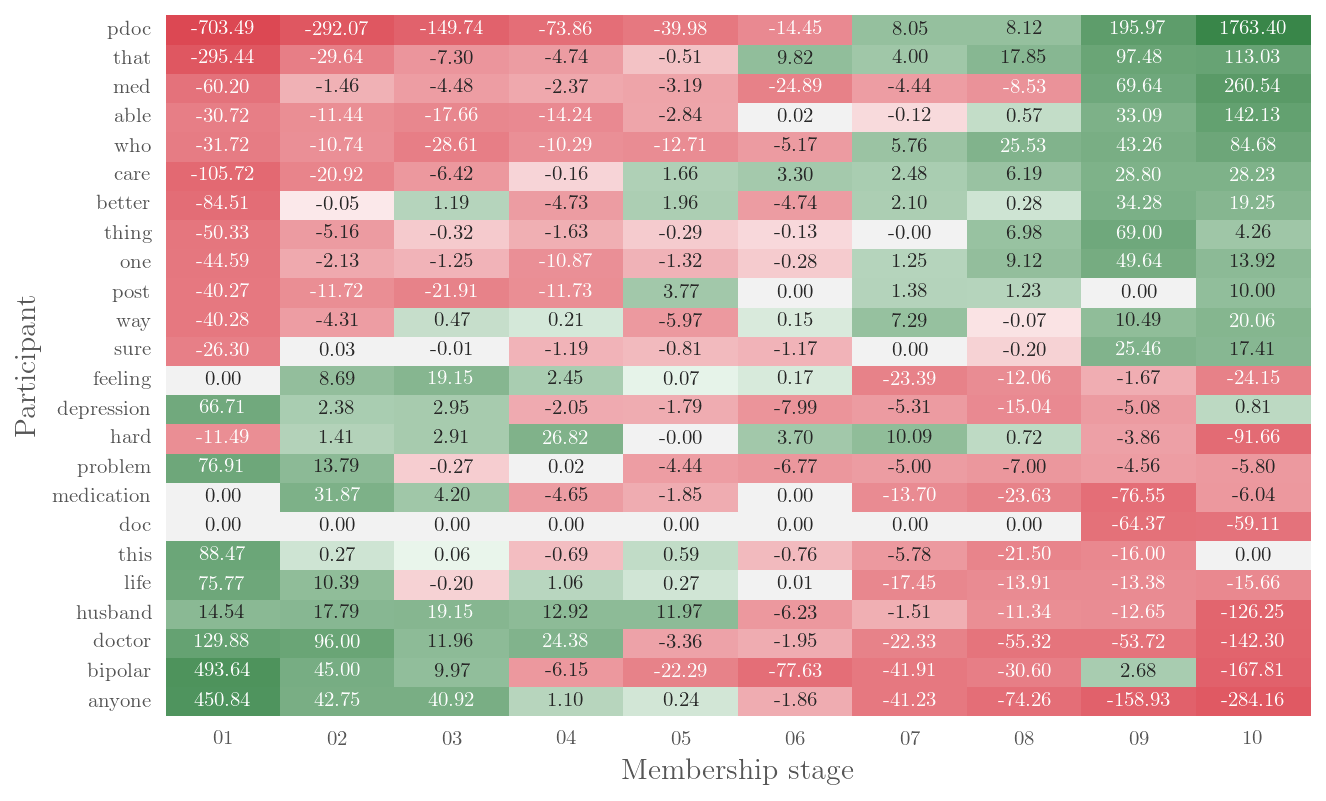
\includegraphics[width=1\textwidth]{../images/symlog-part2}
    \caption[Keywords on increasing and decreasing trajectories]{Keywords on increasing and decreasing trajectories (symmetric logarithmic colour scale)}
    \label{fig:key-traj}
    \end{figure}

Exploratory concordancing of various lexical items in Table \ref{tab:keyunkey-threestage} and Figure \ref{fig:key-traj}, revealed four key \glspl{theme}: \emph{jargonisation}, \emph{metadiscourse}, \emph{vague language} and \emph{the construal of instability}. These \glspl{theme} are explored in the sections below. 

\subsection{Jargonisation} \label{sect:jargon}

% Jargon term use by postcount
\begin{figure}[htb]
    \begin{center}
    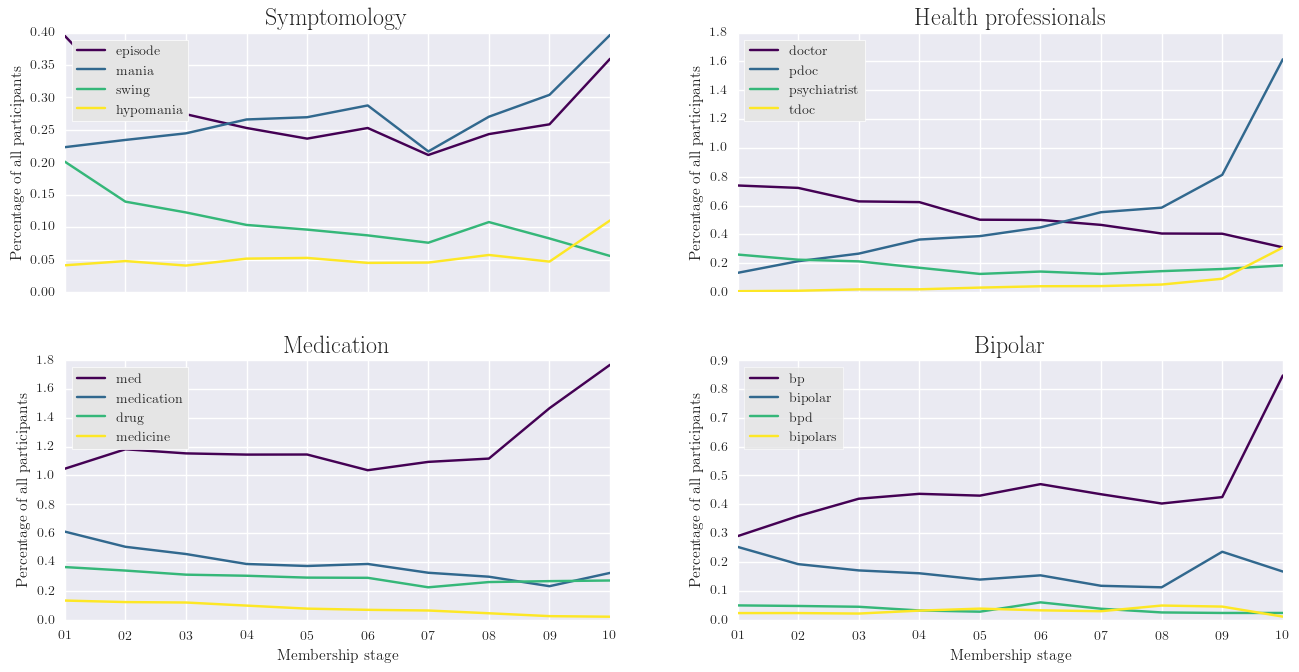
\includegraphics[width=0.90\textwidth]{../images/better_jargon.png}
    \end{center}
    \caption{Jargon term use by postcount}
    \label{fig:jargon}
    \end{figure}

The first theme of interest based on participant frequencies is jargonisation. In systemic\hyp{}functional terms, jargon serves important roles within both interpersonal and experiential metafunctions. Interpersonally, jargon demonstrates familiarity with community norms and expectation \cite{martin_language_2005}, and can demonstrate a (lay) expertise that enhances legitimacy. Experientially, jargon can also achieve more delicate distinctions between important participants in a given Field of discourse: the shift from construal of \emph{mood swings} to states of \emph{mania and hypomania} highlight the potential for jargon to facilitate more advanced taxonomisation of \gls{bipolar} and its symptoms.

Over the course of membership, jargon becomes significantly more common: \emph{meds}, \emph{pdoc}, \emph{tdoc}, \emph{bp} and \emph{mania} are all \gls{Forum} jargon, all featuring and within most key participants in late stages of membership (Table \ref{tab:keyunkey-threestage}) and the top ten participants in veteran \gls{member} talk in terms of relative frequency. Jargon terms also steadily displace non\hyp{}jargon variants: \emph{medication} becomes \emph{med(s)}, and \emph{bipolar} becomes \emph{bp}. Figure \ref{fig:jargon} shows this pattern in four subcomponents of the Field of discourse overall. Within symptomatology, \emph{mood swings} decrease, as discussion of \emph{mania} and \emph{hypomania} emerge. Terms for health professionals are shortened: psychiatrist and doctor become \emph{pdoc} at later stages. For medication, \emph{Med(s)} rises in frequency while \emph{medication} and \emph{drug} decline. For Bipolar Disorder itself, veteran members show a dramatic shift in preference toward \emph{bp}. Interestingly, some changes are multi\hyp{}stage: Figure \ref{tab:key_part_w_prop} shows how \emph{doctor} becomes \emph{doc} in middle stages, before finally splitting into \emph{pdoc} and \emph{tdoc} in late stages.

A final point to note here is that the relationship between participant and lexical item is not perfectly one\hyp{}to\hyp{}one, as many agnate terms (often in the form of jargon) exist at different stages of membership to denote the same Thing. Therefore, to more accurately gauge shifting Fields of discourse, it is necessary to attempt at least a basic collapsing of participant taxonomies, and of jargonised and non\hyp{}jargonised terms. This is performed later in the chapter.

\subsection{Metadiscourse}

% problem: the examples aren't participants!
%todo: help interpreting the figure
As can be seen in Figure \ref{fig:metadiscourse}, \emph{board} and \emph{group} are the main way that members refer to the community itself (0.044 and 0.065 per cent of all participants, compared to \emph{forum} at 0.009 per cent). \emph{Board} and \emph{group} become more frequent over the membership course, as do other terms that denote features of the \gls{OSG} such as \emph{post} and \emph{thread}. While new \glspl{member} typically commend the \glslink{Forum}{board} and explicitly mark the fact that they have recently found it, veteran \glspl{member} speak on its behalf and outline its goals and orientation (see Table \ref{tab:board} for instances of \emph{board}, not limited to participant roles). Over the course of membership, \glslink{member}{users} thus increasingly construe the community as a Thing that can bring about Events and Goals. Most importantly, the \gls{Forum} is capable of acting \emph{for} \glslink{member}{users} in the service of providing information and support. Construal of the \gls{Forum} as a static entity acted upon by its \glspl{member}, or as a non\hyp{}essential circumstance of location, decreases over time.

% Key metadiscourse words
\begin{figure}[htb]
    \begin{center}
    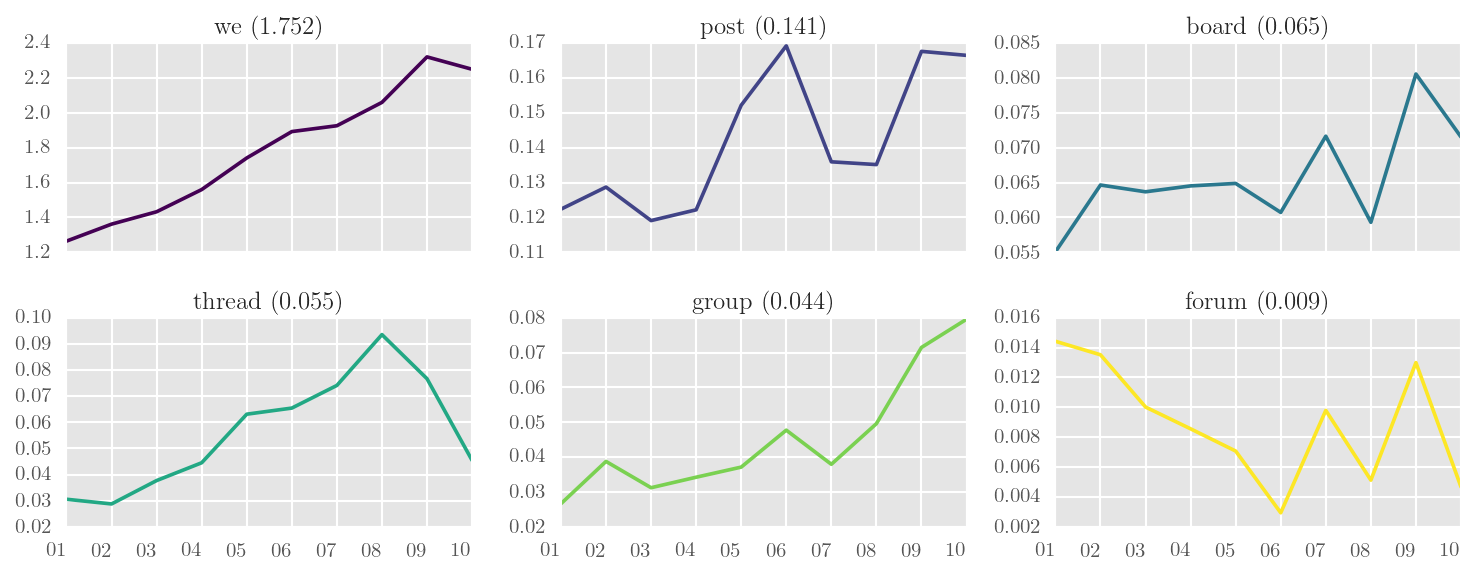
\includegraphics[width=0.70\textwidth]{../images/subplot-metad.png}
    \end{center}
    \caption{Key metadiscourse words}
    \label{fig:metadiscourse}
    \end{figure}


% References to \emph{board} in new and veteran talk
\begin{figure}[htb]
    \centering
    %\minipage{0.44\textwidth}\centering
    \begin{tabular}[t]{@{}>{\raggedright\arraybackslash}p{0.45\textwidth}}
    \vspace{1mm}
    New users
    
    %\noindent\parbox[t]{0.44\textwidth}{\raggedright%
    \begin{enumerate} [before=\itshape,font=\normalfont] \setlength\itemsep{0em} \footnotesize
    %\item Keep talking and being patient ... it will happen but it isn't going to happen overnight like we all would like it too.
    \item I'm so happy to have found this \textbf{board}.
    \item I'm not new to the \lbrack website\rbrack, but new to this \textbf{board}
    \item Thanks for this \textbf{board}, everyone's \glspl{post} have been really helpful to read.
    \item I am hopeful regarding being on this message \textbf{board} and sharing with all of you.
    \item i just joined this message \textbf{board}.
    \end{enumerate}
    \end{tabular}
    \begin{tabular}[t]{@{}>{\raggedright\arraybackslash}p{0.5\textwidth}}
    \vspace{1mm}
    Veteran users
    
    \begin{enumerate}[before=\itshape,font=\normalfont] \singlespacing \setlength\itemsep{0em} \footnotesize
    \item I'm glad you told him about the \textbf{board} and about NAMI.
    \item Part of the purpose of the \textbf{board} is for venting.
    \item Hello, Welcome to the \textbf{board}.
    \item on this \textbf{board} at least , pdoc is psychiatrist and tdoc is shorthand for therapist...
    \item Your sage comments are missed by all on the \textbf{board}.
    \end{enumerate}
    \end{tabular}
    %\endminipage
    \caption{References to \emph{board} in new and veteran talk}
    \label{tab:board}
    \end{figure}
%
\noindent Though experiential meanings, strictly speaking, construe information about events in the world, rather than role\hyp{}relationships between participants in interactions \cite{eggins_introduction_2004}, salient role\hyp{}relationship negotiation is performed through the differing discursive function of metadiscourse according to membership length. New \glspl{member}' discussion typically highlights the division between the \glslink{Forum}{community} and the self (\emph{I'm so happy to have found this board}), whereas veteran \glspl{member} construct a shared identity with the \glslink{Forum}{board} (\emph{Hello, welcome to the board}). Further, only veteran talk about the board is elaboratory or explanatory (\emph{Part of the purpose of this board is for venting}).

Also shown in Figure \ref{fig:metadiscourse} is that the use of \emph{we} increases over the course of membership. Concordancing of Subcorpus 10 shows that \emph{we}, like \emph{board} and \emph{group}, commonly occurs during explanation of the function(s) of the \glslink{Forum}{community} to newer \glspl{member}. As can be seen in Figure \ref{fig:we_conc}, another common use of \emph{we} in veteran talk is in generalisations about the lived experience of all people living with \gls{bipolar}---a discursive strategy that simultaneously stakes a claim to knowledge about bipolar and highlights the role of lay\hyp{}experience as the source of this knowledge.

%Two functions of \emph{we} in veteran users' language
\begin{figure}[htb]
    \centering
    %\minipage{0.44\textwidth}\centering
    \begin{tabular}[t]{@{}>{\raggedright\arraybackslash}p{0.45\textwidth}}
    \vspace{1mm}
    \begin{enumerate} [before=\itshape,font=\normalfont] \singlespacing \setlength\itemsep{0em} \footnotesize
    \item Hang in there and know that \textbf{we} are all rooting for you.
    \item Keep on venting and taking one thing at a time and know that \textbf{we} are here.
    \item So what happened, {[}username{]} ... \textbf{we} were soo worried about you the other night.
    \item None of us can diagnose you since \textbf{we} are n't medical professionals, but it very well could be bipolar.
    \item Also remember that \textbf{we} are all here for you anytime you need us.
    \end{enumerate}
    \end{tabular}
    \begin{tabular}[t]{@{}>{\raggedright\arraybackslash}p{0.45\textwidth}@{}}
    \begin{enumerate}  [before=\itshape,font=\normalfont] \singlespacing \setlength\itemsep{0em} \footnotesize
    \item For whatever reason, \textbf{we} want to think that the brain \textbf{we} were born with is just fine thank you very much.
    \item With bipolar disorder the rock does edge off of us - it just seems to take forever and \textbf{we} are so powerless beyond our meds to make it go away.
    \item I think sometimes \textbf{we} are just too overwhelmed to act.
    \item I think part of the reason \textbf{we} crash is that \textbf{we} are simply exhausted.
    \item For after all, \textbf{we} are all the sum total of our experiences.
    \end{enumerate} 
    \end{tabular}
    \caption{Two functions of \emph{we} in veteran users' language}
    \label{fig:we_conc}
    \end{figure}

\subsection{Vague language} 

The appearance of \emph{thing} as an increasingly prominent participant in veteran talk warranted further analysis. Initially, lemmatisation had conflated \emph{thing} and \emph{things}, with the latter being the site of the most change. Concordancing of \emph{things} in new \gls{member} \glspl{post} showed that \emph{things} often described past circumstances (\emph{things were getting really bad}). In contrast, veteran \glspl{member} used \emph{things} in expressions of general support (\emph{things will get better!}): % (see Figure \ref{fig:things}). 

%todo
%things as subject as perc of subjects / things not as subject as perc of non-subjects
% things as subject in present tense / things as subject in past tense

% things
\begin{enumerate} [before=\itshape,font=\normalfont] \singlespacing \setlength\itemsep{0em} \footnotesize
    %\item   \textit{\textbf{things} will get better}
    \item  I hope  \textbf{things} improve for you soon
    %\item  I really hope \textbf{things} go well for you
    \item  I am glad that  \textbf{things} are looking up for you too
    \item  call your pdoc if  \textbf{things} do not improve very soon!
    %\item  put on a brave face during the times when \textbf{things} seem so great
    \item  decided to hold off a semester until you get \textbf{things} more under control
    %\item  Let us know how  \textbf{things} go.
    %\item  perhaps it will be your opportunity to turn \textbf{things} around
    \item  as soon as you get back on your meds \textbf{things} will be better, just wait and see!!!
    %\item  want to run away thinking that it will make  \textbf{things} better
    \end{enumerate}
%
To measure this difference, the tenses of clauses in which \emph{things} takes the position of experiential subject (generally Actor, but, more rarely, Sayer, Senser, or Token\slash Possessor) in new and veteran \glspl{member}' \glspl{post} were tallied. Figure \ref{fig:thingstense} shows that \emph{things} is more commonly used by new \glspl{member} to describe action in the past. In veteran talk, \emph{things} tends to be vague, and is more commonly focussed on the present and future. This change echoes the more general shift toward present tense, as outlined in the previous chapter. Though more in\hyp{}depth analysis is perhaps warranted, this feature in veteran talk could potentially be a strategy for providing advice that may be of benefit to the entire \glslink{Forum}{community}, rather than simply the \gls{thread} initiator. An alternative analysis is that \emph{things} may allow veterans to provide social support without the need to ask follow\hyp{}up questions. Given the high dropout rate of new \glslink{member}{users}, with most new \glslink{member}{users} \glslink{post}{posting} fewer than three times, requests for clarification of specific circumstances may often go unanswered. In order to complete more exchanges, advice is accordingly dispensed as soon as possible, with little clarification sought. Another manifestation of this strategy can be seen in Emz's reply to a new member in Chapter \ref{chap:introdata}: rather then attempting to clarify unexplained parts of the newcomers' narrative, Emz instead simply highlights that her beliefs and suggestions are based on incomplete information (\emph{From what you say, if sounds very likely that you might have Bipolar disoder}; \emph{If you're already seeing a psychiatrist [...], then find a different one}).

% Tense of clauses with \emph{things} as subject by postcount
%\begin{figure}[htb]
%    \begin{center}
%    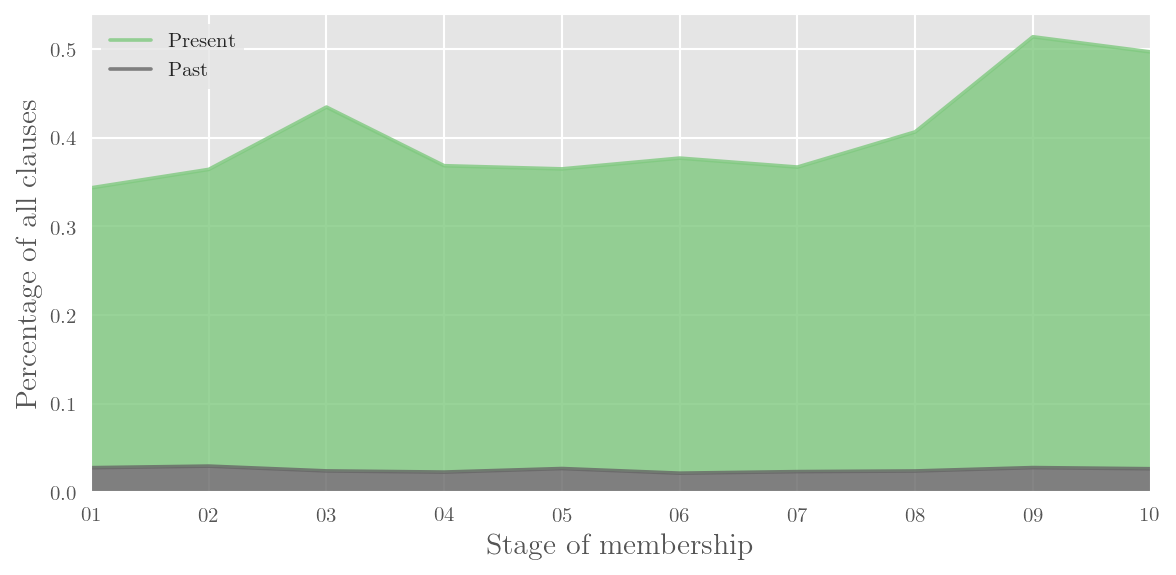
\includegraphics[width=0.70\textwidth]{../images/tense-things-new-area.png}
%    \end{center}
%    \caption{}
%    \label{fig:thingstense}
%    \end{figure}

\begin{figure}[htb]
    \minipage{0.48\textwidth}\centering
    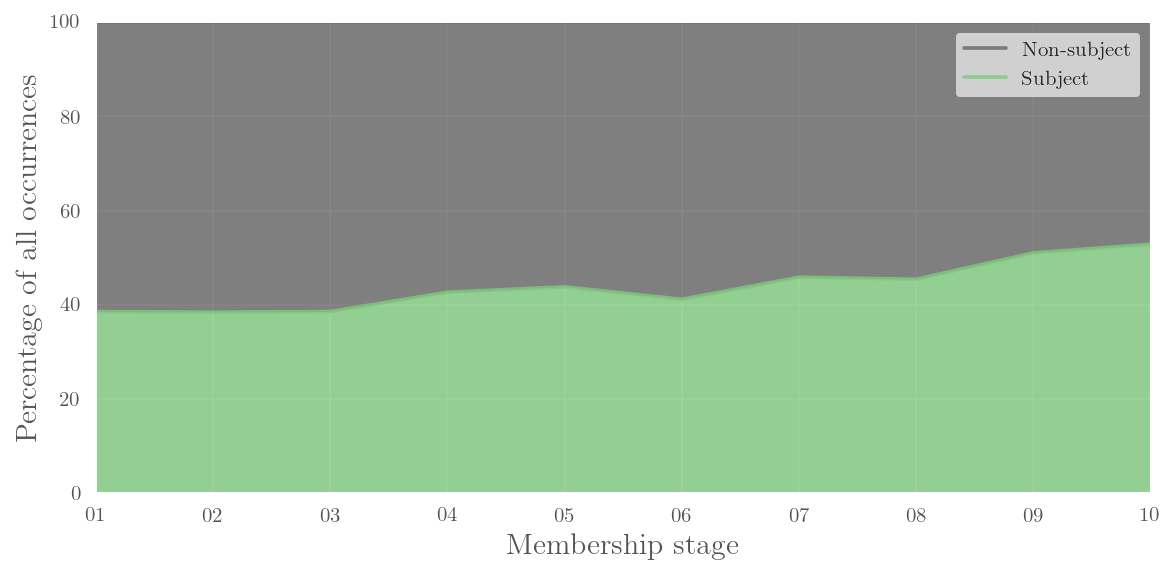
\includegraphics[width=1.00\textwidth]{../images/things-area.png}
    \endminipage\hfill
    \minipage{0.48\textwidth}\centering
    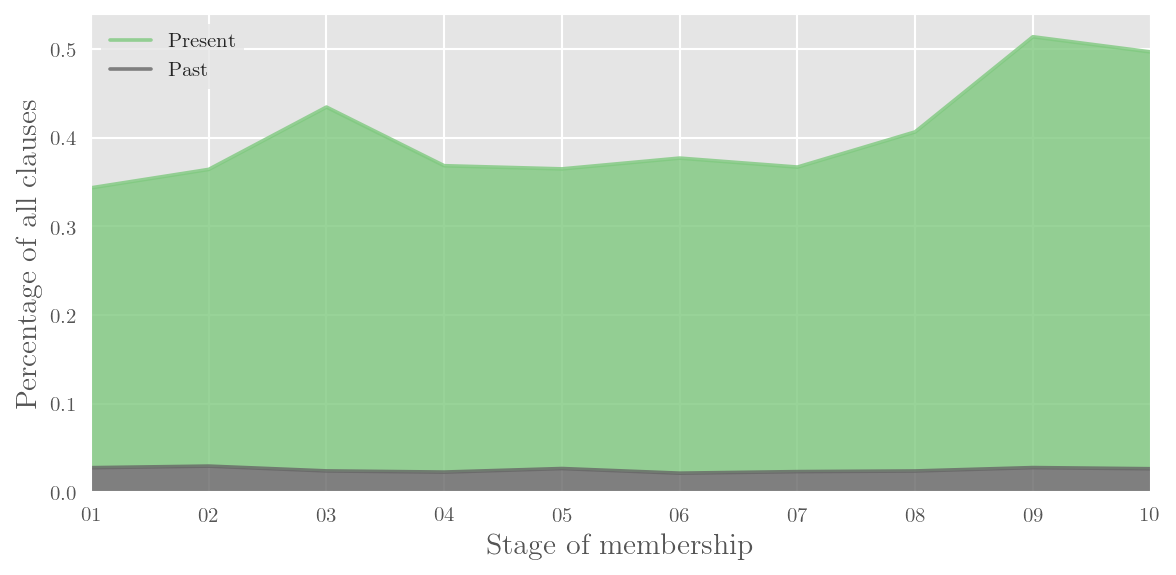
\includegraphics[width=1.00\textwidth]{../images/tense-things-new-area.png}
    \endminipage\hfill
    \caption[Increasing use of \emph{things}]{\emph{Things} as an increasingly common left participant, and as an increasingly common left participant in present tense clauses}
    \label{fig:thingstense}
    \end{figure}

\FloatBarrier
\subsection{Construing (in)stability}

Other results highlight changes in experiential semantics that can be mapped to the ideological orientation of the \glslink{Forum}{community}. One striking pattern evident in Table \ref{tab:keyunkey-threestage} is that newer \glspl{member} commonly construe negative mental states and desires that index instability and volatility (\emph{swing, angry, scared, crazy, kill}, etc.). For veterans, such terms are unkey, being reconfigured under an attitudinally neutral or potentially medicalised nominalisation, \emph{imbalance}. As seen in the qualitative analysis and noted in related literature \cite[e.g.][]{horne_doing_2009}, new \glspl{member} produce medical narratives connoting urgency in order to legitimate their membership bid and elicit responses. The framing of bipolar symptoms in emotive language, however, is dispreferred, with veteran \glspl{member} avoiding attitudinal lexis in favour of a nominalisation, \emph{stability}, which is represented as the possible result of proper care.

\begin{table}[htb]
\centering
\begin{tabular}{rll}
\toprule
terms of making sure that she finds &  stability   &  .                                   \\
t your finding and maintaining your &  stability   &  as well .                           \\
are important as far as maintaining &  stability   &  .                                   \\
to try different avenues to achieve &  stability   &  .                                   \\
            that way you will reach &  stability   &  so much quicker .                   \\
 those of us who have finally found &  stability   &  for ourselves or our loved ones it  \\
lf so that you will be able to find &  stability   &  and identify the stressors and deve \\
               he has given me more &  stability   &  over 2 months than i 've had in 1.5 \\
our `` seasoned '' bper who has had &  stability   &  for over 35 years .                 \\
 between of something resembling `` &  stability   &  '' or `` normalcy . ''              \\

\bottomrule
\end{tabular}
\caption{\emph{Stability} in veteran posts}
\label{conc:stability}
\end{table}

%\endnote{Tregex queries: \thingspresent~ and \thingspast}~ %A final point of discussion here is the appearance of \emph{things} in the top participants in veteran talk (See Figure \ref{fig:things}). The abstract and interpretable nature of the term (like \emph{time}, \emph{years}, \emph{people} and \emph{life}) allows it to be easily applied to the circumstances of newcomers when, especially when many details aren't known to the veteran member

\subsection{Construing human agency}

%todo: flag methodology
Because jargonisation disperses the potential lexical realisations of participants, wordlists must be created that can collapse the distinction between participants with multiple realisations in lexis during the \gls{corpus} interrogation process. The main human participants \cite[or social actors---see][]{van_leeuwen_representation_1996} in the Field of discourse can be divided into four : \emph{The Self}, \emph{Other Members}, \emph{Friends\slash Family} and \emph{Health Professionals}, with wordlists developed to match jargonised and non\hyp{}jargonised variants (Table \ref{tab:hum_part_lex_real}). For the remainder of the thesis, these capitalised terms denote the results of the four search queries, while lowercase variants refer to the social actor in general. Of course, such an approach means that many instances will go uncaptured, due to grammatical metaphor, misannotation, pronominalisation and so on. Even so, there is sufficient data for exploring how these four participant types behave over the membership course. Figure \ref{fig:part-tax-rel-freq} shows the relative frequency of four kinds of human participants over time. Clearly, Other \glspl{member} come to steadily displace the self as the ideational social actor being represnted. Friends and family, meanwhile, are on an uneven trajectory, occupying a larger part of the semantic space in early and late stages of membership than in the middle. Construal of health professionals rises dramatically in the late stages of membership. %The findings concerning Self and Other are in line with previous interrogation results. Collapsing jargon variants of terms for health professionals, however, has allowed us to see the overall rise in construals of health professionals as participants over the membership course. 

\begin{table}[htb]
    \centering
    \small
    \begin{tabularx}{\textwidth}{lX}
    \toprule
    Participant type & Realisations \\ \midrule
    The Self                & \emph{i}, \emph{myself}, \emph{me}            \\
    Other Members           & \emph{you}, \emph{yourself}, \emph{kat}, \emph{seaturtle}            \\
    Friends\slash Family    & \emph{friend}, \emph{mother}, \emph{husband}, \emph{daughter}, \emph{son}, \emph{wife}, \emph{father}, \emph{dad}, \emph{mom}, \emph{mum}, \emph{erin}           \\
    Health Professional     & \emph{doc}, \emph{docs}, \emph{doctor}, \emph{doctors}, \emph{dr}, \emph{dr.}, \emph{drs}, \emph{g.p.}, \emph{gp}, \emph{gps}, \emph{nurse}, \emph{nurses}, \emph{pdoc}, \emph{pdocs}, \emph{psych}, \emph{psychs}, \emph{shrink}, \emph{shrinks}, \emph{tdoc}, \emph{tdocs}           \\ \bottomrule
    \end{tabularx}
    \caption{Human participants and lexical realisations}
    \label{tab:hum_part_lex_real}
\end{table}

\begin{figure}[htb]
    \centering
    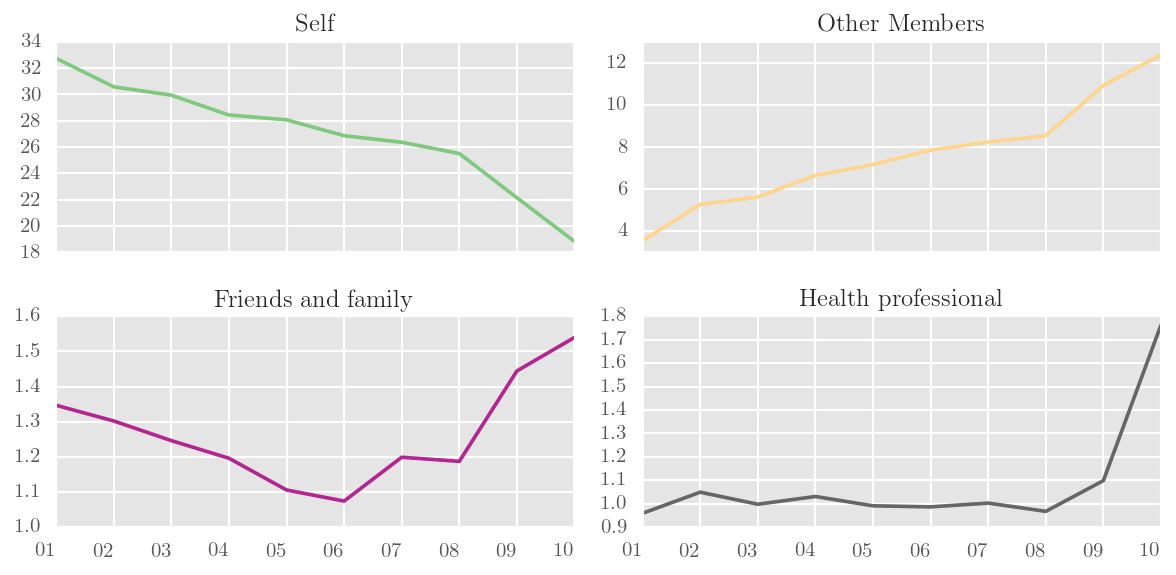
\includegraphics[width=0.8\textwidth]{../images/part-tax-rel-freq.png}
    \caption[Frequencies for four participant types]{Relative frequency of four participant types over the course of membership}
    \label{fig:part-tax-rel-freq}
    \end{figure}

Next, the ergative model of \sctext{Transitivity} can be used to determine the extent to which these human participant types are construed as Agents, and how this shifts with membership length. To measure this, each occurrence of participant type occuring in an Agentive dependency role can be divided by occurrences of the same participant type filling any participant role (Figure \ref{fig:key_proc_for_parts}). This controls for differences in the overall frequency with which certain participant types are mentioned.

Most notable in Figure \ref{fig:key_proc_for_parts} is the wide gap between health professionals and non\hyp{}health professionals in early contributions: when professionals are mentioned as participants in first \glspl{post}, they are in positions of experiential agency over 75 per cent of the time. Non\hyp{}health professionals, on the other hand, are more commonly positioned as Media---that is, as the entity through which a process comes into being. This is a representation of a world where health professionals are granted more control over medical processes than healthcare \glspl{consumer}, and where change in the world is enacted through the consumer, who may be willing or unwilling: patients are treated by doctors; doctors tell patients how to manage their condition. 

The clearest individual trend is the increasing agency granted to \gls{Forum} \glspl{member} generally. Veteran \glslink{member}{users} construct a discourse of \gls{consumercentred}ness by positioning their interlocutors as able to actively make changes in their inner and outer states. This method also makes it possible to see, for the first time, an increasing agency of The Self within the Field of discourse. Though The Self is less often charged with ensuring the completion of the clause as an intersubjective proposition (a responsibility increasingly delegated to the addressee), The Self is increasingly positioned as an entity that can bring about change in the world. Finally, there is a modest decrease in the proportion of \emph{Health\hyp{}professional\hyp{}as\hyp{}Agent} over membership length, closing an ideological divide present in early contributions, where health professionals carry out processes through the medium of the sufferer.

\begin{figure}[htb]
    \centering
    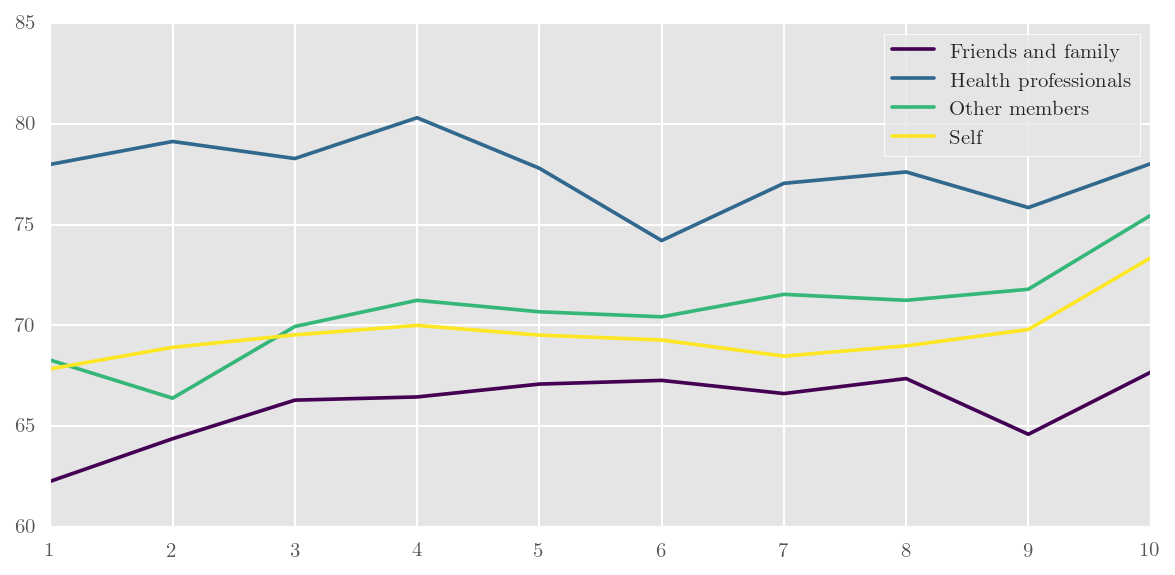
\includegraphics[width=0.85\textwidth]{../images/percentage-agent.png}
    \caption{Proportion of each participant type in Agent role}
    \label{fig:key_proc_for_parts}
    \end{figure}

%The notion of left-participant, however, is semantically very muddy, as participant roles are conflated. This is an unfortunate consequence of the fact that the Universal Dependency grammar does not distinguish between Agent and Medium, except in rare cases, such as passives with a \emph{by}-headed PP.

\section{Key processes} 

The next focus of the analysis of \sctext{Transitivity} choices is on processes, as typically realised by verbal groups at least one nominal group argument. Initially, we are interested in the head of this Process, which corresponds to the Event in the \gls{SFG}. In a constituency grammar, this is generally the rightmost verb in a VP; in the Universal Dependency grammar, Events are annotated with \emph{ccomp}, \emph{cop}, \emph{advcl} and \emph{root} labels. Therefore, an analysis of processes can begin in the same way that the analysis of participants was carried out, but with process\hyp{}like labels substituted for participant\hyp{}like ones.

% Key and unkey Events in each subcorpus
\begin{figure}
    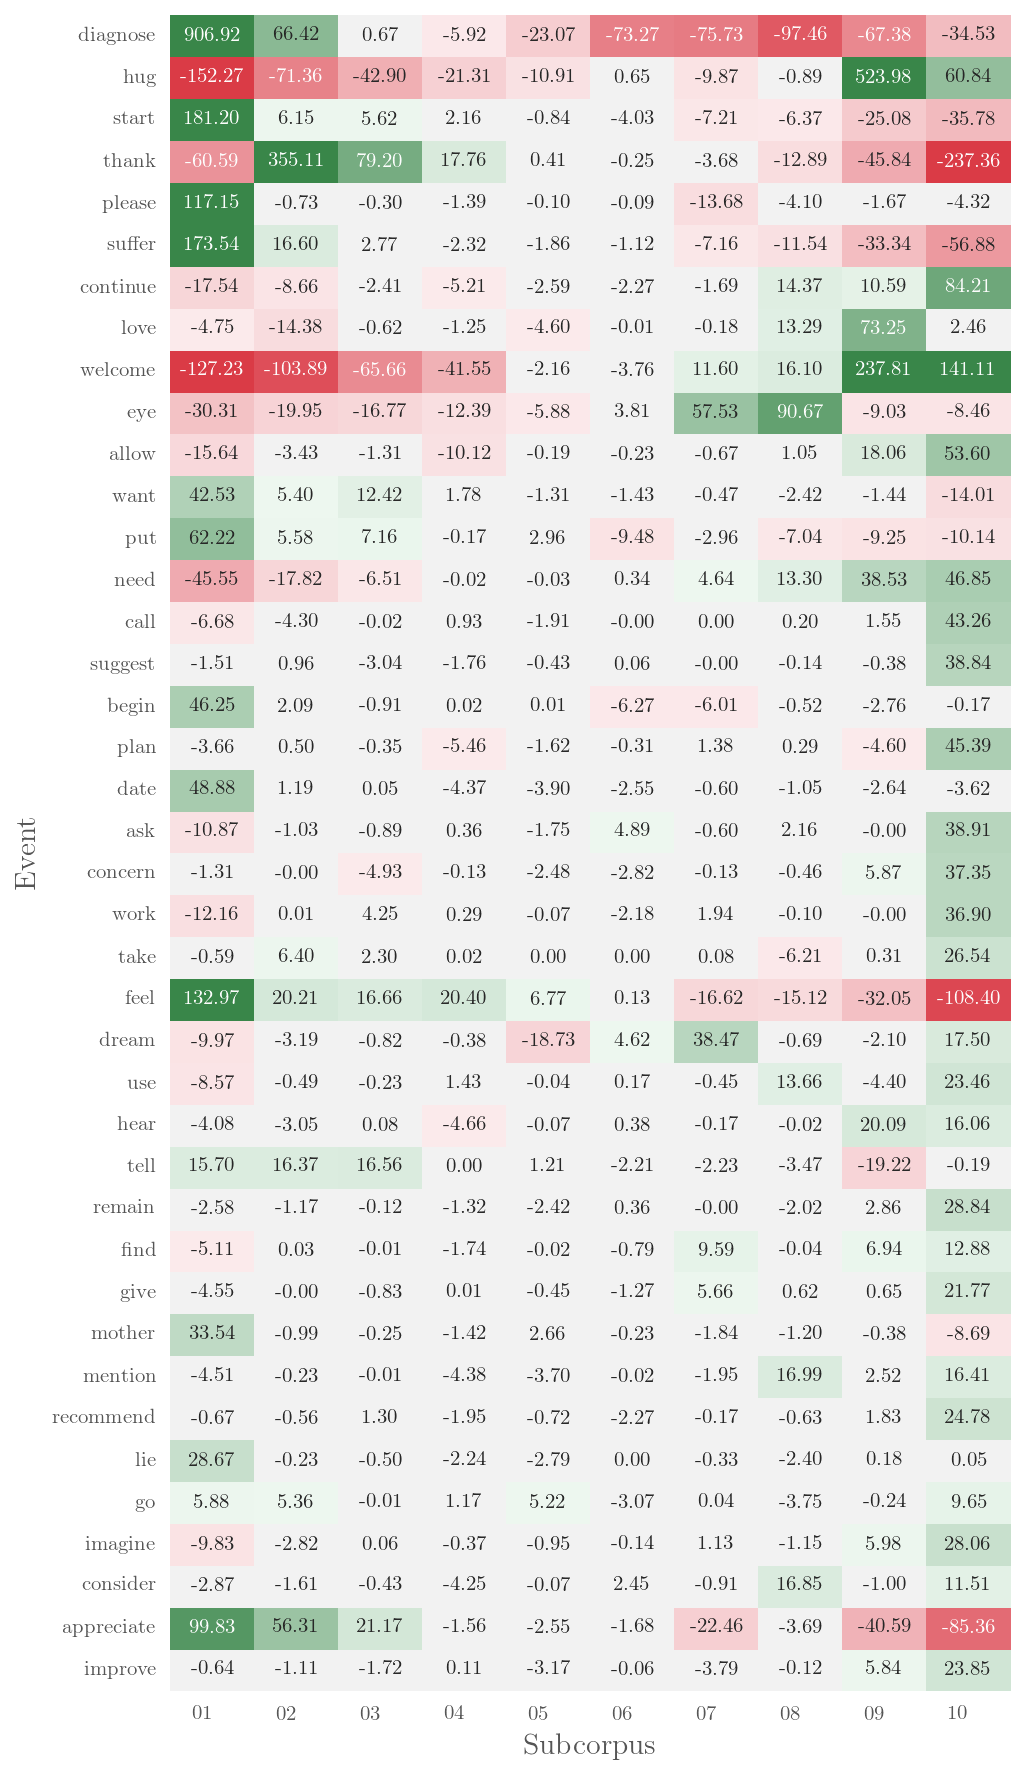
\includegraphics[width=0.80\textwidth]{../images/event-heatmap.png}
    \hspace{1.6cm}
    \caption{Key and unkey Events in each subcorpus}
    \label{fig:event_heatmap}
    \end{figure}

Figure \ref{fig:event_heatmap} shows which Events are key in each subcorpus according to a log\hyp{}likelihood comparison of the \gls{Forum} contents as a whole. By far the most key process in any subcorpus is \emph{diagnose} in Subcorpus 01, as diagnosis is both the catalyst for visits to the site, and the main entry condition for participatory information and support exchange. Similarly, \emph{thank} is key in second \glspl{post} because \glslink{member}{users} thank others for replies to their first. Other key Events in first \glspl{post} reveal other kinds of motivations for joining the \glslink{Forum}{community}, including being \emph{told} that they may have \gls{bipolar}, \emph{dates} with \glslink{bipolar}{bipolar} people, and \emph{beginning\slash starting} new medication regimens or manic\slash depressive cycles.

As with the analysis of participants, where veteran \glspl{member} orient toward more positive lexis, positive processes related to social support also become more common in veteran \glspl{post} (\emph{hug, thank, love, welcome}). Another focal point is processes urging others to carry on (\emph{continue, remain, improve}), which also have positive connotations. This contrasts with the negative sentiments inherent in \emph{suffer} (as in, \emph{to suffer from bipolar}), which is key in first \glspl{post} (see below for a more thorough treatment of the ways in which bipolar is ascribed to the self and others across membership stages). Finally, it is notable that \emph{thank} and \emph{appreciate} are unkey in the final stage of membership; the increased social status in the \glslink{Forum}{community} means that platitudes, for veterans, are no longer obligatory to the same extent.

\subsection{Construing diagnosis} \label{sect:diag}

%Concordancing allows a window into the figures involving \emph{diagnose} in early and late stages of membership.

% Goal of \emph{diagnose} processes in three stages of membership
% Circumstances in \emph{diagnose} processes in three stages of membership
\begin{figure}[htb]
    \centering
    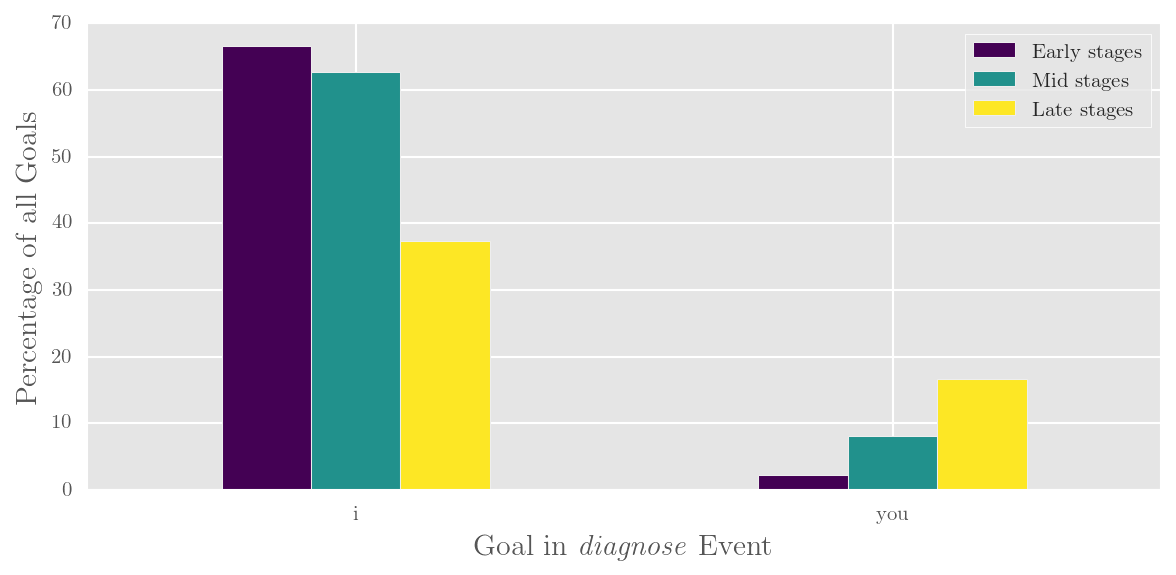
\includegraphics[width=0.8\textwidth]{../images/goal-in-diag-ev.png}
    \caption[Goal of \emph{diagnose} processes]{Goal of \emph{diagnose} processes in three stages of membership}
    \label{fig:part_in_diag}
    \end{figure}

    \begin{figure}[htb]
    \centering
    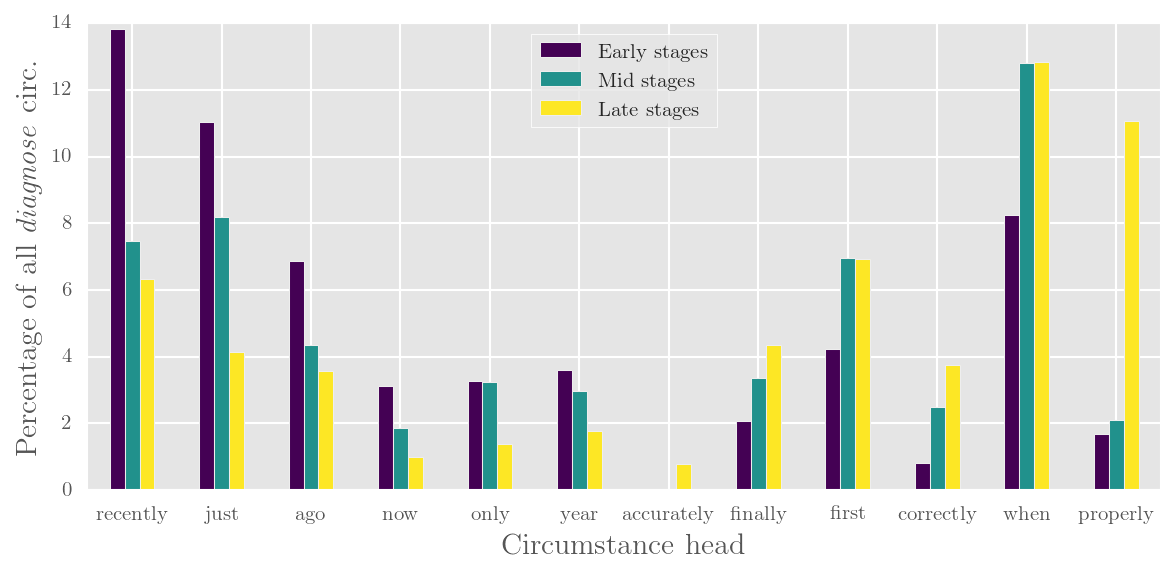
\includegraphics[width=0.8\textwidth]{../images/diag-circ.png}
    \caption[Circumstances in \emph{diagnose} processes]{Circumstances in \emph{diagnose} processes in three stages of membership}
    \label{fig:circ_in_diag}
    \end{figure}

\emph{Diagnose} is a very prominent process in the \gls{Forum}, and is by far the most key of key processes expressed in first \glspl{post}. By contrasting early, middle and late stages of membership, clear differences emerge in how the process of diagnosis is configured over time (Figure \ref{fig:part_in_diag}). Veteran \glspl{member}, for example, are more likely to represent the health professional as the Actor in the \emph{diagnose} process. In terms of circumstances (Figure \ref{fig:circ_in_diag}), there is a shift in focus away from temporal meanings, with veteran \glspl{member} instead framing the \emph{diagnose} process with regard to its correctness, accuracy and legitimacy. New \glspl{member} often enter the community because of a recent or possible future diagnosis. Veterans, on the other hand, seek to ensure that the diagnosis is reliable. This has the dual purpose of ensuring the legitimacy of the new member's `entry ticket', and ensuring conformance with the biomedical model, where successful treatment is predicated on accurate diagnosis. Indeed, a number of \glslink{member}{users} enter the community not because of a diagnosis from a health professional, but because they are attempting to ascertain whether their self\hyp{}diagnosis, or their informal diagnosis of a friend or loved one, can stand up to the scrutiny of lay\hyp{}experts. Veteran members, however, are reluctant to legitimise these kinds of strategies, due to their deviation from a normative conceptualisation of the `correct' consumer journey.

%Furthermore, they frame diagnosis as possibilistic: diagnoses can be \emph{suspected} or \emph{unofficial}. Such a framing is at odds with the normative biomedical model, however: informal kinds of diagnosis cannot be acted upon with appropriate treatment regimens. Veteran \glspl{member} therefore stress correct diagnosis in order to realign new \glspl{member}' construal of diagnosis with the ideology of the \glslink{Forum}{board}.

%Though the focus of the community is on offering information and support for people with \gls{bipolar}, those without official diagnoses ultimately cannot be helped \cite{vayreda_social_2009}. Ideologically, validation of community membership is withheld until new members have aligned with a normative biomedical trajectory that foremost involves diagnosis by professionals operating within a formal healthcare institution.

Notably, veteran \glspl{member} may deliberately undermine the biomedical model of diagnosis. While expressing conviction that diagnosis must be performed by a qualified health professional, they may simultaneously hint that the newcomer is \emph{probably} bipolar, or that non\hyp{}bipolar diagnoses are in error. As was shown in the qualitative analysis in Chapter \ref{chap:introdata}, two separate replies to an undiagnosed newcomer relied upon the same lexicogrammatical means of hinting (\emph{It sounds like you might have bipolar to me}; \emph{if sounds very likely that you might have Bipolar disoder}), while nonetheless insisting on seeking diagnosis through mainstream channels (\emph{Find you a dr that can make a correct Diagnosis}; \emph{We aren't docs here and can't diagnose you}). As shown in the following section, in veteran--veteran interactions, health professionals' ability to correctly identify and treat people living with \glslink{bipolar}{bipolar} is occasionally into question. This keeps the membership entry point open for those who have initially failed to meet the core criterion of a legitimate diagnosis, while pushing undiagnosed, suspected \glslink{bipolar}{bipolar} \glslink{member}{users} toward actions that are in line with mainstream medical norms. %Help can be better provided once the condition is met.

\subsubsection{Diagnosis and grammatical metaphor}

Grammatical metaphor entails the use of one grammatical component to do the work that is congruently performed by another. Nominalisation is one of the most common examples \cite{simon-vandenbergen_grammatical_2003}. What is congruently an action, process or Event (e.g. to \emph{applaud}) may be reconstrued as a participant (\emph{applause}), allowing denser packaging of information. Turning the process into a participant also facilitates taxonomisation and classification: the lexical component of a nominal group may include Classifier, Epithet and Numerative, in addition to the Thing; in the verbal group, the only lexical component is the Event \cite{halliday_introduction_2004}. This kind of grammatical metaphor also opens up the reconstrued process to deixis. For these reasons, it is a key characteristic of scientific English \cite{halliday1999construing}. 

Over the course of membership, the process of diagnosis undergoes a steady shift toward metaphorical realisation as a participant. In formal terms, it is more often nominalised. Figure \ref{fig:diag-gram-met} shows the strong relationship, but inexact, relationship between nominalisation and grammatical metaphor in the case of diagnosis: nominal and participant realisations become more frequent, while verbal and process realisations decrease. Charting experiential roles shows us that \emph{diagnose} is not limited to participant and process roles: commonly, it is a part of a circumstance (\emph{we received more help in terms of diagnosis and treatment}) or modifies a Thing (\emph{it is extremely common for those with undiagnosed bipolar disorder to self medicate}). The increasing extents to which \emph{diagnose} is nominalised, and to which \emph{diagnose} is represented as something other than a process, demonstrate an important discourse-semantic shift. By moving away from \emph{diagnose\hyp{}as\hyp{}process}, it becomes possible to represent diagnosis as a possession, (\emph{it's great you have a final diagnosis and have started medication}), and therefore something that can be acted upon or thought of in a particular way (\emph{i finally feel like i've accepted my diagnosis}). Another possibility opened up by nominalisation is the potential for modification through Epithets (\emph{this is a frightening diagnosis, particularly if you don't know anyone who has it}). Classification of \emph{diagnosis} through adjectival modification is also made possible (\emph{accurate}\slash \emph{correct} diagnosis), but, of course, as shown in Figure \ref{fig:circ_in_diag}, agnate meanings can be made through circumstantial modification of diagnose as a process (\emph{accurately\slash correctly diagnosed}). A final grammatical affordance is that diagnosis as a participant in a relational process can highlight its potential to be incorrect (\emph{my current diagnosis is schizo\hyp{}affective disorder}; \emph{bp is becoming a catch-all diagnosis, frequently made by a well-meaning family doctor}). In this way, grammatical metaphor not only contributes to an increasingly scientised register, but also expands veteran members' ability to explain medical processes and their relationship to other members \cite{heyvaert_nominalization_2003}.

Calculating the relative frequencies of common modifiers of diagnose as verb (\emph{diagnose}, \emph{diagnosed}, \emph{diagnosing}) and diagnose as noun (i.e. diagnosis\slash diagnoses) clearly shows a preference for temporal modification of verbs and veracious modification of the nominal form.

%More generally, veterans may wish to invoke a scientised register, which 

% Grammatical metaphor in \emph{diagnosis}, via word classes and experiential roles
\begin{figure}[htb]
    \minipage{0.48\textwidth}\centering
    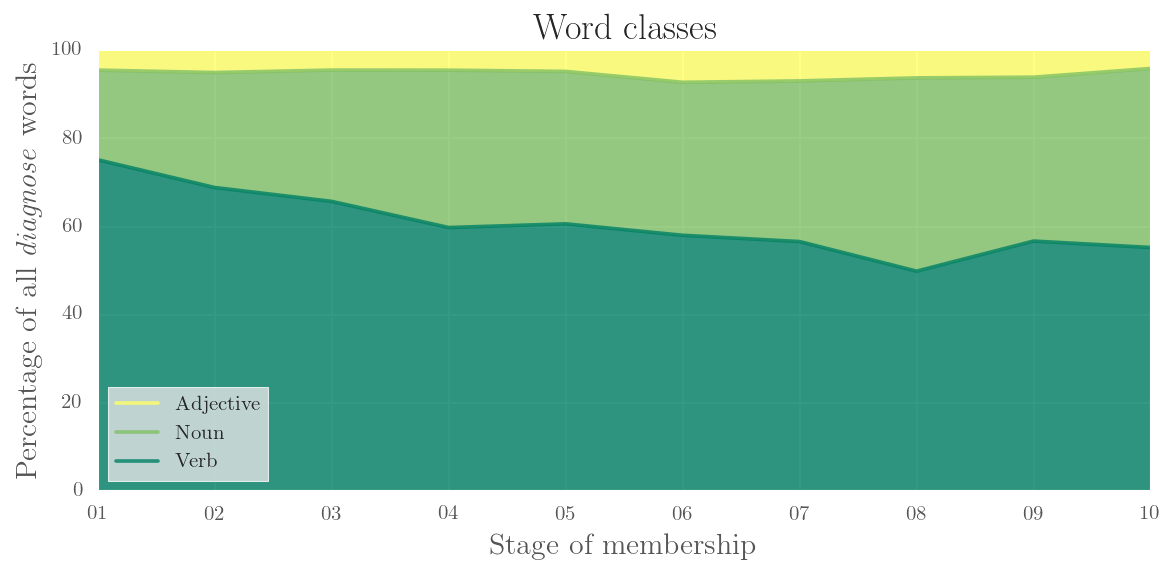
\includegraphics[width=1.00\textwidth]{../images/wc-diag.png}
    \endminipage\hfill
    \minipage{0.48\textwidth}\centering
    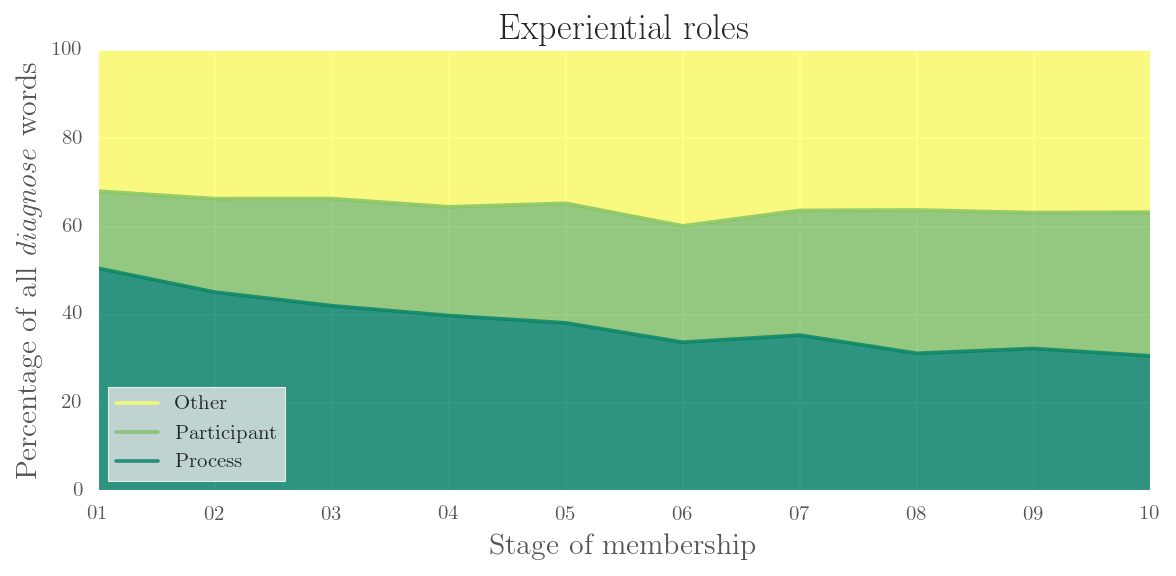
\includegraphics[width=1.00\textwidth]{../images/exp-diag.png}
    \endminipage\hfill
    \caption[Grammatical metaphor in \emph{diagnosis}]{Grammatical metaphor in \emph{diagnosis}, via word classes and experiential roles}
    \label{fig:diag-gram-met}
    \end{figure}

\begin{table}[htb]
\begin{tabular}{lrlr}

\toprule
\emph{Diagnose}  & Rel freq.        & \emph{Diagnosis} & Rel. freq. \\
\midrule
not               &  11.80 & bipolar    &  11.13 \\
ago               &  11.10 & proper     &   8.82 \\
just              &   7.60 & correct    &   7.49 \\
recently          &   6.68 & dual       &   5.07 \\
when              &   4.16 & right      &   4.41 \\
now               &   3.54 & new        &   3.96 \\
only              &   3.11 & official   &   2.75 \\
properly          &   2.75 & different  &   2.64 \\
also              &   2.27 & wrong      &   2.20 \\
finally           &   2.12 & other      &   2.20 \\
so                &   2.09 & same       &   1.87 \\
never             &   2.09 & initial    &   1.65 \\
then              &   1.93 & possible   &   1.54 \\
correctly         &   1.50 & true       &   1.54 \\
well              &   1.47 & recent     &   1.43 \\
\bottomrule
\end{tabular}
\caption{Most common modifiers of \emph{diagnose} and \emph{diagnosis}}
\label{relfreq-diagnose-mods}
\end{table}

%As could be expected, diagnosis is increasingly construed as a participant in the \Gls{forum}. By calculating the relative frequency of the diagnose process compared to processes generally, of diagnosis participants compared to participants generally, and diagnose words within other experiential roles, compared to other roles generally, we can see that diagnosis

% Interpretation?

\subsection{Construing the relationship between people and bipolar} \label{subs:behave}
    
As noted by \textcite{harvey_disclosures_2012}, people attribute depression to themselves in a number of different ways. The same set of grammatical constructions are available to those afflicted by many health issues, including \gls{bipolar}. In the \glslink{Forum}{Bipolar Forum}, people may \emph{have}, \emph{be}, \emph{feel} or \emph{suffer from} bipolar. For reasons of scope, however, only the two most common clause-level ascriptions---\emph{having} and \emph{being}---are examined in detail here, and group\slash phrase level ascriptions (i.e. \emph{a bipolar friend}) are not considered. To look for longitudinal changes in being\slash having constructions, the \gls{corpus} was interrogated for relational processes with bipolar (or jargon variants \emph{bp, bpi, bpii, bp1, bp2}, etc.) as a first object argument, and with human pronouns as the leftmost nominal group, returning lemma forms of the located relational Events.\endnote{Searching for participants by their order in clauses is often inaccurate, due to passivisation. In the case of relational processes, however, this is not an issue, as relational processes cannot be passivised (\emph{*bipolar was suffered from by me}).} Generated concordance lines were used to remove false positives caused by parser errors. Results were then recalculated from the concordance lines using \texttt{corpkit}'s \texttt{Concordance.calculate()} method.

%Lemmatisation was used to collapse the verb inflections for \emph{be}, \emph{have} and \emph{suffer}. Two kinds of false positives were discounted. First, clauses with \emph{it} as subject were excluded, as they were not ascribing bipolar to people, but explaining that bipolar is the cause of a certain symptom (e.g. \emph{It's probably the bipolar that makes you do that}).

% Processes with bipolar as Medium, combined
% Processes with bipolar as Medium, separated
\begin{figure}[htb]
  \begin{center}
  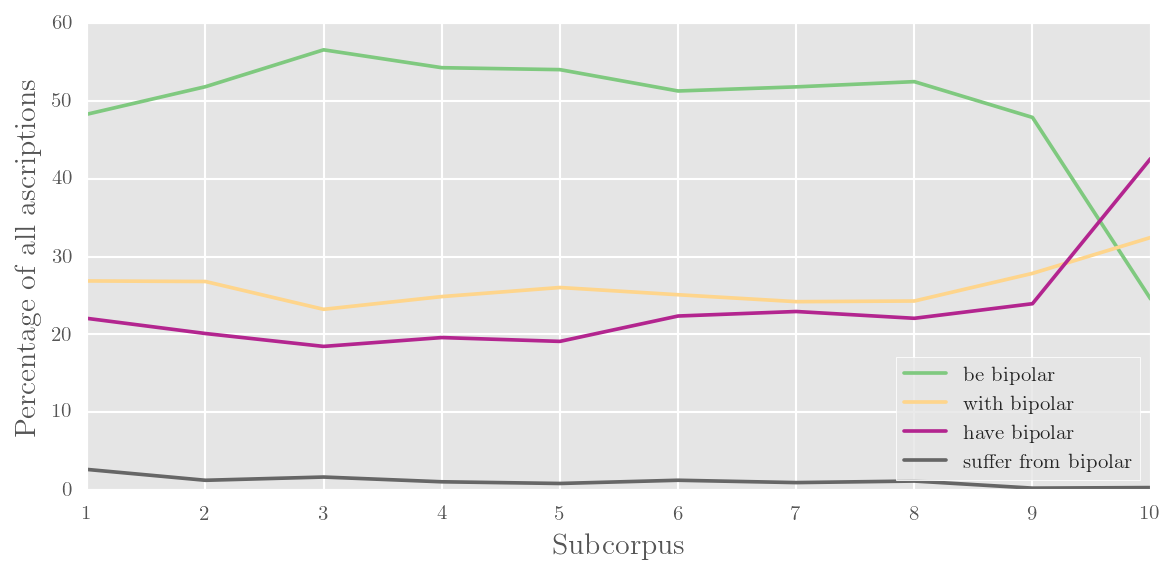
\includegraphics[width=0.75\textwidth]{../images/being_having.png}
  \end{center}
  \caption{Processes with bipolar as Medium, combined}
  \label{fig:behave}
  \end{figure}

  \begin{figure}[htb]
  \begin{center}
  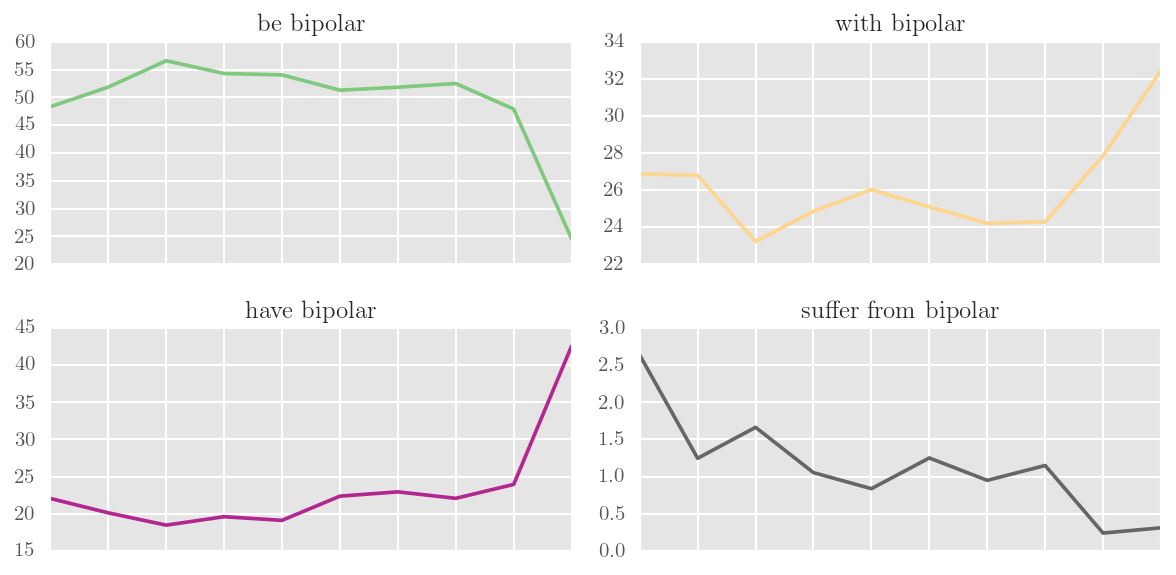
\includegraphics[width=0.75\textwidth]{../images/being_having_subplots.png}
  \end{center}
  \caption{Processes with bipolar as Medium, separated}
  \label{fig:behave_subplot}
  \end{figure}

Figures \ref{fig:behave} and \ref{fig:behave_subplot} show changes in the way \gls{Forum} \glslink{member}{users} construe the relationship between bipolar, themselves and others. Most strikingly, \emph{having} forms overtake \emph{being} forms as ways of ascribing \gls{bipolar} to the self and others. This change occurs very late in the membership course. Similar is the growth in attribution via circumstances, as in \emph{a person with bipolar}. To \emph{suffer from} \glslink{bipolar}{bipolar} decreases steadily over the course of membership.

Understanding these changes requires analysis of the grammatical properties of each kind of ascription. First, the shift away from \emph{suffering from} and \emph{feeling} is away from mental and toward relational processes. This shift includes the increasing frequency of attribution via \emph{with}, as grammatical circumstances are in fact partially articulated relational processes. Both \emph{being} and \emph{having} constructions are attributive relational processes, meaning that in both cases an attribute is ascribed on some level to the experiential subject. The difference is in the nature of the attribution. \emph{I have bipolar} is a \textbf{possessive attributive}, in which the experiential subject functions as a possessor of the attribute, which is inherently possessed. Possession itself is foregrounded in the process of having; ownership of bipolar is ascribed to the subject. Inversion of the clause highlights the dominance of the possessor over the possessed: \emph{bipolar has me} conveys an (undesirable) lack of control over the condition. \emph{I am bipolar}, on the other hand, is an \textbf{intensive attributive} construction, where bipolar forms a class in which the subject is a member. Halliday and Matthiessen's \citeyear{halliday_introduction_2004} use of the term \emph{Carrier} for the subjects in these kinds of processes highlights the ambiguity concerning the Carrier's willingness to be ascribed the attribute. This construct is ultimately dispreferred by veteran users, as it creates a subclass of person characterised chiefly by the ascribed bipolarity, rather than foregrounding the process of ownership, and, by extension, some control over their possessed condition.

The salience of the two constructions is evident in the fact that veteran \glslink{member}{users} of the \emph{Bipolar Forum} may explicitly draw attention to the \emph{being\slash having} distinction. Recalling the qualitative analysis of a new \glslink{member}{user}'s interaction with two more senior \glspl{member} (see Section \ref{sect:jess-post} for the complete reproduction), we can see that each interactant construes Jess as having \gls{bipolar} using different relational process lexis:

\begin{quotation}\small\singlespacing

\noindent \textbf{Jess}: [...] i have asked my doctor to test me to see if i am bipolar as my antidepressants do not work even though they have been changed a million times!! [...] i want to change my doctor and have been telling my partner i would but im scared of finding out that i am bipolar [...]

\noindent \textbf{Luvsoccer}: It sounds like you might have bipolar to me. You need to change Drs. One with more knowledge apparently. The reason the antidepessants are not Working is because If you are bi polar and they put U on an antidepressant alone it can make things worse... [...]

\noindent \textbf{Emz}: Hi, welcome to the boards, hopefully we can help you out and be a support system for you. First off you're not A bipolar, *l* we're not things, it's a condition. From what you say, if sounds very likely that you might have Bipolar disoder. [...]

\end{quotation}
%
Jess exclusively uses \emph{being} forms, while \emph{Luvsoccer} switches between \emph{having} and \emph{being}. Emz, however, uses only \emph{have} forms, except when explicitly drawing attention to the fact that copula ascription is dispreferred. To make this point, she highlights a potential reading of the \emph{being} construction as an \emph{intensive identifying} process, whereby the experiential subject has \emph{bipolar} assigned to it for the purposes of identification, rather than quality attribution. This is undesirable among the community: as explained by the veteran user, it is preferable to be a member of a class of \emph{people} possessing a particular quality of \emph{bipolar}, rather than a relationship of equivalence between the Identifier and Identified.

% A veteran user discussing the being\slash having distinction
\begin{figure}[htb]
  \centering
  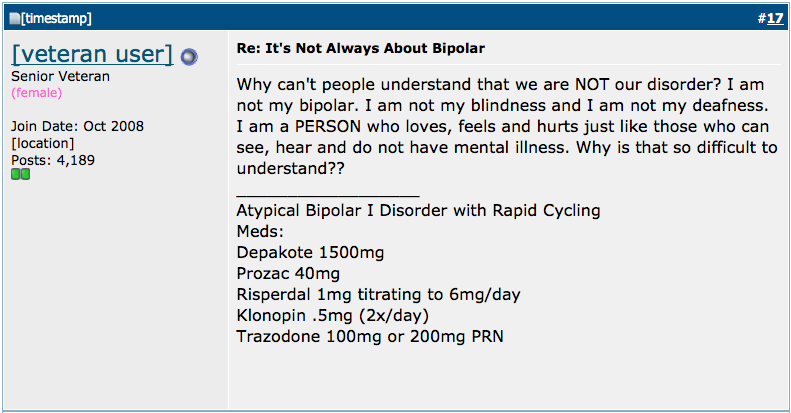
\includegraphics[width=0.60\textwidth]{../images/notourbipolar.png}
  \caption{A veteran user discussing the being\slash having distinction}
  \label{fig:notour}
  \end{figure}
%    
Some of the rare instances of \emph{being} constructions in Subcorpus 10 are in fact the result of veteran \glslink{member}{users} recasting new users' claims of \emph{being bipolar} as \emph{having bipolar}, as can be seen in Emz' response to Jess. Note the veteran's insertion (and capitalisation) of the indefinite article during her recast: \emph{First off, you're not \textbf{A} bipolar, we're not things}. Here, the veteran \gls{member} is highlighting a second potentially undesirable reading of the \emph{being} construction, where rather than functioning as an Epithet, \gls{bipolar} becomes a Thing. This transforms the attribute into an entity, rather than Quality, and renders the class of \glslink{bipolar}{bipolar} (as the veteran \gls{member} points out) a Thing to which a person can be equated, rather than a trait that may (currently) characterise someone.

%% Veteran recasting new user's copula constructions
%\begin{figure}[htb]
%  \begin{center}
%  \includegraphics[width=1.0\textwidth]{../images/newandreply.png}
%  \end{center}
%  \caption{Veteran recasting new user's copula constructions}
%  \label{fig:notabipolar}
%  \end{figure}

%Genre analysis (see below) suggests that new members' introductions to the community may be influenced by prior knowledge of generic norms in face\hyp{}to\hyp{}face support groups, such as \emph{Alcoholics Anonymous}, in which members use a well-known \emph{being} form when greeting one another (\emph{Hi, I'm \lbrack ~name \rbrack~ and I'm an alcoholic}). Though this influences the prevalence of being forms in first \glspl{post}, \emph{being} forms persist during the first stages of membership (see Figure \ref{fig:behave}).

Aside from recasts, in veteran \glspl{post}, however, \emph{being} constructions are exceptionally rare. In the highest postcount group, only 11 matches were found, with eight cases involving ascription to others, rather than the writer him\slash herself. One post, in which the self was identified as \emph{being} \glslink{bipolar}{bipolar} three times was selected for further analysis (Figure \ref{fig:firstsaid}).
    
%\endnote{The AA website explains that `Using the somewhat cliched AA introduction of ``Hi, my name is \lbrack name\rbrack~and I'm an alcoholic'' is not requirement but simply a custom adopted independently by many groups and members' \citeyear{_must_2014}}~
%\begin{quote}
%\small \singlespacing
%The pdocs at the first hospital said I was bp1. Then at the state hospital they said I was bp2, then they said I was schizoaffective bipolar type.
%\end{quote}

% A veteran user employs \emph{being} forms
\begin{figure}[H]
  \begin{center}
  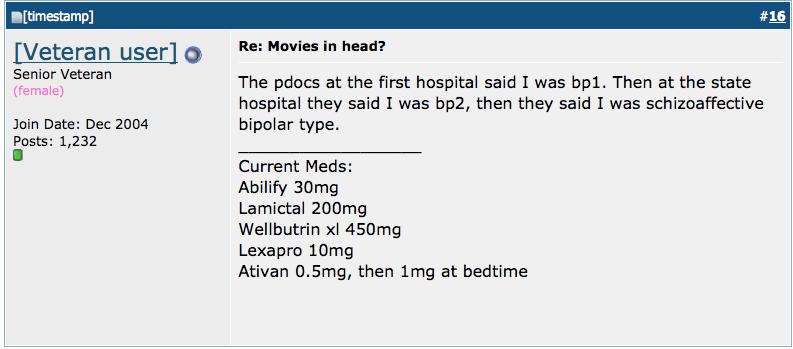
\includegraphics[width=0.6\textwidth]{../images/firstsaid.png}
  \end{center}
  \caption{A veteran user employs \emph{being} forms}
  \label{fig:firstsaid}
  \end{figure}
%
\noindent Here, pivotally, it is pdocs, rather than the speaker himself, who (twice) invoke the \emph{being} construction, through an embedded clause in the Verbiage. Given that elsewhere in the forum the same member had employed \emph{having} constructions, analysis of entire threads was performed, in order to better understand veteran's motivations for using \emph{being} forms. In multiple cases, veterans appeared to use \emph{being} constructions to help establish a negative characterisation of the health professionals in the process of diagnosis. In an earlier \gls{post}, the \glslink{member}{user} had told the story of his misdiagnosis:
    
            %\begin{quote}
            %\small \singlespacing
            %If you can't be hypomanic and have psychosis, then why in the hospital did they change my diagnosis to bipolar 2 when I was clearly psychotic? They changed it that way because they said I have more problems with depression instead of mania. That was their reasoning.
    
            %\noindent Now my diagnosis is something different. I'm beginning to wonder if some of these pdocs even know what they are doing.
            %\end{quote}

% A veteran user's characterisation of pdocs as incompetent
\begin{figure}[H]
  \begin{center}
  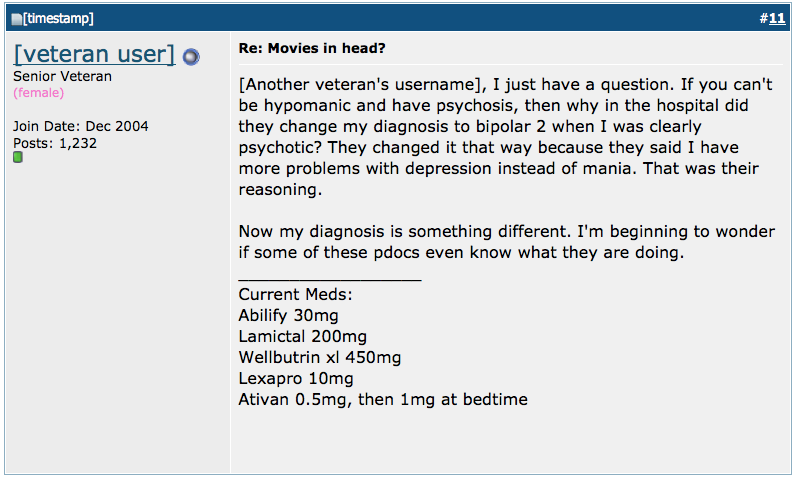
\includegraphics[width=0.6\textwidth]{../images/incomppdocs.png}
  \end{center}
  \caption{A veteran user's characterisation of pdocs as incompetent}
  \label{fig:incomppdocs}
  \end{figure}
%
\noindent The writer's uses of the dispreferred \emph{being} constructions add weight to his positioning health professionals as incompetent: in the narrative, health professionals can neither offer correct diagnosis for their patients nor adequately conceptualise the relationship of ownership and possession between person and condition that functions as an important normative value in the \glslink{Forum}{community}.

\subsection{Process-participant type configurations}

Earlier, I analysed the frequency of four kinds of participants in the Forum's Field of discourse (\emph{The Self}, \emph{Other Members}, \emph{Health Professionals} and \emph{Friends\slash Family}, and the proportion of occurrences of each participant within the role of Agent (within an ergative interpretation of the system of \sctext{Transitivity}). The transitive interpretation of the system can be used to investigate the processes each Agent is involved in. Figure \ref{fig:key_proc_for_parts2} visualises the keyness of lexical heads of processes.

% Four participant and process types
% Keyness of processes involving four participants
\begin{figure}[htb]
  \centering
  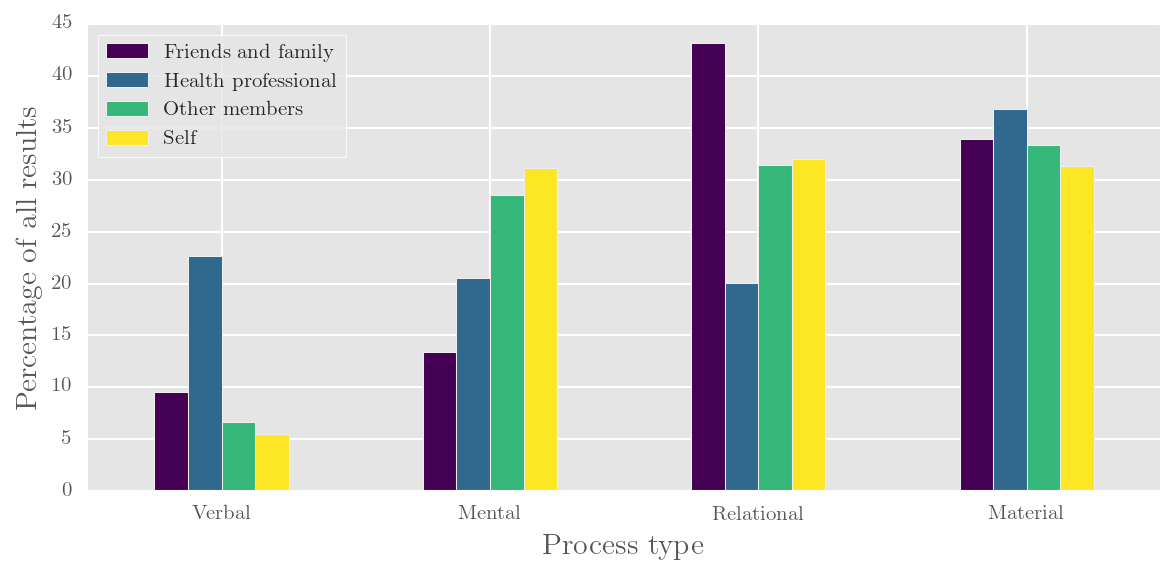
\includegraphics[width=0.80\textwidth]{../images/process-types-for-part-types.png}
  \caption{Four participant and Process Types}
  \label{fig:process-types-for-part-types}
  \end{figure}

  \begin{figure}[p]
  \centering
  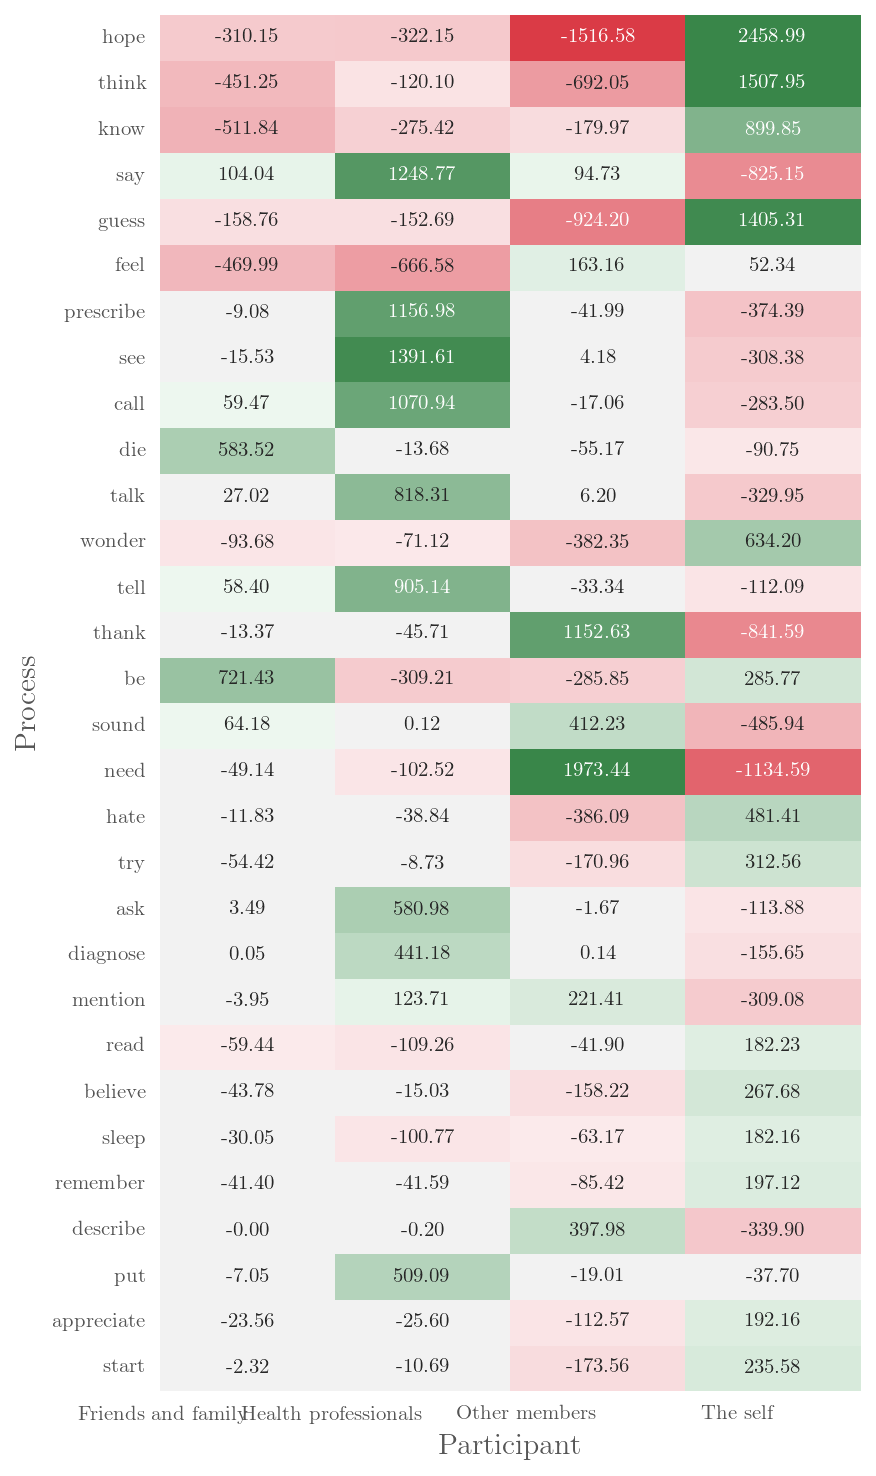
\includegraphics[width=0.80\textwidth]{../images/left_participant_in.png}
  \caption{Keyness of processes involving four participants}
  \label{fig:key_proc_for_parts2}
  \end{figure}

Finally, the individual processes can be collapsed by Process Type (Figure \ref{fig:process-types-for-part-types}). A four-type system, as described in the Cardiff Grammar, is used here, due simply to the availability of the Process Type Database \cite{neale_more_2002}. Processes are defined broadly. \emph{Feel} and \emph{smell}, for example, are counted within both \emph{mental} and \emph{relational} types (though they could be differentiated by counting the number of participants). As the Process Type Database did not contain some common processes found in the \gls{corpus} (e.g. \emph{diagnose}), the top 200 processes in the \gls{corpus} were added to lists manually if absent based on intuition and grammatical tests. Material processes are simply those that do not occur in the other three lists.

It can also be observeed that different participant types are typically construed as participating in different kinds of activities. Health professionals are most commonly Sayers, as language is the means through which mental health treatment is predominantly provided. Diagnosis, elicitation of symptoms, prescription, advice, referral, and most kinds of therapy are accomplished through talk. The Self is positioned as a Sayer far less often: speakers do not construe their own speaking within the Field of discourse, because speakers' talk is primarily an interpersonal, rather than an experiential phenomenon; its function is to enact and negotiate with the addressee.

Mental processes of thinking and feeling are most commonly performed by the Self. This is perhaps expected, because \glslink{member}{users} have unmediated access to their own thoughts; others' mental processes are often accessed through other Process Types. Other members are commonly construed as Sensers in irrealis scenarios, and\slash or during the provision of advice or health information (see Table \ref{conc:others-in-mental}). Formulaic or idiomatic expressions such as \emph{if you know what I mean} and \emph{you know} also play a role. Rarely, however, do veteran \glspl{member} construe newcomers' manic\slash depressive episodes.

% Other members as Senser in veteran posts
\begin{table}[htb]
  \centering
  \small
  \begin{tabular}{ll}
  
  \toprule
  $1660$ &  you do n't want him taking something that effects the chemstry of his brain  \\
  $1370$ &  do you know what has helped me with self-esteem ?                                                \\
  $4064$ &  i know how you feel about your son being on such strong medications .                            \\
  $4827$ &  you have to be responsible in letting your pdoc know that your meds are n't working  \\
  $2125$ &  you just have to find what helps you the best .                                                  \\
  $4327$ &  i hope that you will find the program very beneficial .                                          \\
  $632 $ &  you have to train your mind to allow alot of this external stimuli to bounce off  \\
  $4401$ &  all will be okay , and it will be over before you know it .                                      \\
  $1111$ &  you have come to the right place to learn about your disorder , to find support  \\
  $3018$ &  can you help me understand why you can only contact your pdoc 1 time per month ?                 \\
  \bottomrule
  \end{tabular}
  \caption{Other Members as Senser in veteran posts}
  \label{conc:others-in-mental}
  \end{table}

Friends and family, meanwhile are most commonly represented within relational processes. Two reasons for this are that many \glslink{member}{users} enter the \glslink{Forum}{community} seeking a classification of a friend\slash family member's symptoms as being or not being consistent with \gls{bipolar}. Relational processes are the congruent grammatical means of performing such classificatory work. Another reason is that friends and family are construed through sequences of relational processes that function as a statement of medical history and demographics. In the example below, the new user describes her son and his actions via a sequence of relational processes, with the son in the position of Token. The text concludes by relating both her son and Self to \Gls{bipolar} using an Identifying relational.

% i'm the mother of 3 sons ...
\begin{quote}
\small
\singlespacing
I'm the mother of 3 sons. My middle son \textbf{is} our problem. Ugh, problem isn't even close to the appropriate word. But, I guess I'll go with that. Where to start............as of now he\textbf{'s} a chronic runaway, self medicates, he\textbf{'s been} in trouble with the law, He spent 72 hours in the psych ward as a 5150 for threatening to kill himself, his emotions are up and down, he\textbf{'s} nasty, hateful, on the other hand loving and warm. Towards me in particular, he blames me for everything and says if he\textbf{'s} bipolar so am I. 
\end{quote}
%
This brief account of participant and Process Type constellations is a useful place to conclude the case study analysis. On one hand, the findings challenge Widdowson's (\citeyear{widdowson_limitations_2000}) argument that \gls{CL} reveals findings contrary to expectation: we would expect that the Self is more likely to be construed as engaging in mental processes, simply because humans have constant access to their own thoughts. Likewise, we would also expect friends and relatives to be construed relationally (so that addressees understand the role of third parties in the discourse), and pdocs to provide diagnosis and treatment through talk. The expectedness of results is, foremost, an indication that the methods presented are capable of automatically developing an account of discourse that is not at odds with intuition. At the same time, however, the role of the discourse analyst has not been erased: the subtle distinctions made within and across individual \glspl{post} often elude search queries; the mapping of what is found automatically to what can be found through close reading remains, for now, well beyond the power of computational tools and methods.

\section{Chapter summary}

In this chapter, I have analysed \sctext{Transitivity} choices in the \gls{Forum}, and how they change longitudinally. By progressing from frequency and keyness calculations of participants and processes toward analysis of salient items and their syntagmatic behaviour, I showed how \gls{Forum} members construe the world differently at different stages of membership. In the next chapter, I discuss the findings presented in the previous three chapters, mapping lexicogrammatical changes to \glspl{discourse-semantic}, and relating both to findings of the body of literature reviewed in Chapter \ref{chap:onlinehealth}.

%\subsection{Verbal processes}
%
%Also of interest are verbal processes, and the kinds of participants that occur therein. As noted in the previous section, verbal processes %commonly appear as advice in veteran talk. From this we can find out who is doing the saying, and who is spoken to. We can understand saying %as a kind of agency. Though perhaps a simplification, we can conversely understand the Receiver is less active.
%
%% Theme in Verbiage by Process
%\begin{figure}[htb]
%  \centering
%  \includegraphics[width=0.80\textwidth]{../images/verbproc.png}
%  \caption{Theme in Verbiage by Process}
%  \end{figure}

%\todo{Still to come---I basically want to break down the constituents of the Verbiage, and make a comment about the fact that the structure of Verbal processes is linked to Mood.}
